\documentclass{article}

\usepackage[utf8]{inputenc}
\usepackage[spanish]{babel}

\usepackage{caratula}

\usepackage{subcaption}
\usepackage{graphicx}
\usepackage{subfig}
\usepackage{dirtytalk}
\usepackage{enumerate}

\usepackage{amssymb}
\usepackage{mathtools}
\usepackage{amsmath}
\usepackage{amsthm}

\usepackage{algorithm}
\usepackage{algpseudocode}
\usepackage{listingsutf8}

\usepackage{float}
\floatplacement{figure}{h!}

\usepackage{geometry}
\usepackage{fixltx2e}
\usepackage{wrapfig}
\usepackage{cite}
\usepackage{dsfont}

\usepackage[space]{grffile}

\geometry{
 a4paper,
 total={210mm,297mm},
 left=30mm,
 right=30mm,
 top=30mm,
 bottom=30mm,
 }
 
\newtheorem{theorem}{Teorema}[section]
\newtheorem{corollary}{Corolario}[theorem]
\newtheorem{lemma}{Lema}[theorem]
 
\theoremstyle{definition}
\newtheorem{definition}{Definición}[section]
 
\theoremstyle{remark}
\newtheorem*{remark}{Observación}
 
\begin{document}
% Estos comandos deben ir antes del \maketitle
\materia{} % obligatorio

\titulo{Trabajo Práctico 1}
\subtitulo{}
\grupo{}

\integrante{Bayardo Julián}{850/13}{julian@bayardo.com.ar} % obligatorio
\integrante{Cuneo Christian}{755/13}{chriscuneo93@gmail.com} % obligatorio 
\integrante{Fosco Martín Esteban}{449/13}{mfosco65@gmail.com} % obligatorio 
\integrante{Germán Pinzón}{475/13}{pinzon.german.94@gmail.com}
 
\maketitle

\pagebreak

\tableofcontents

\pagebreak

\section{Introducción}

En el presente trabajo se analizan diversos aspectos de la red utilizando Scapy y se distinguen algunos componentes de la misma utilizando un enfoque formalizado a través del uso de la teoría de la información.

En primer lugar, planteamos un criterio para la identificación de routers IPv4 en redes de área local basándonos únicamente en paquetes ARP interceptados de la red.

En segundo lugar, se presentarán cuatro experimentos realizados sobre distintas redes (tres de ellas redes no controladas y una red casera), consistentes en observar el tráfico de las mismas, intentar comprender la topología de la red, y comprobar la eficiencia de el criterio propuesto.

Finalmente, presentaremos las conclusiones y lecciones aprendidas a partir de los mismos.

\subsection{Criterio de distinción}

Primero, recapitulemos sobre el funcionamiento de ARP en una red IPv4. ARP es un protocolo orientado a la resolución de addresses de hardware a partir de addresses IP: cuando un host A pretende comunicarse con otro host B dentro de la misma red de área local, precisa de la MAC address del host B para poder enviar el paquete al destino; de por sí, ningún host poseé esta información sobre ningún otro host y, por ende, precisamos de una metodología para obtenerla.

En el caso de ARP, esto se realiza a través de dos paquetes enviados sobre IP: los ARP Whois y ARP Is At. En el primer caso, el host A precisa saber el MAC address de B, y por ende envía un paquete de este tipo, donde los campos de source de Ethernet e IP serán los de A, y el MAC address destino será FF:FF:FF:FF (address de broadcast para Ethernet), y el IP address de destino será el IP con el que A quiere comunicarse. 

Para distinguir tanto protocolos como nodos en la red, vamos a centrarnos en observar los gráficos que nos muestran la información (en términos de teoría de la información) que provee una Destination IP Address y tomar la IP que menos información tenga. De esta manera, estaremos quedandonos con el nodo que más apareció en el destino de los paquetes ARP que capturamos. Para distinguir protocolos vamos a hacer lo mismo, es decir quedarnos con el protocolo de menor información y dicho protocolo va a ser el que más fue utilizado.

\subsection{Aclaraciones sobre la recolección y análisis de datos}
Para la presentación de los datos se decidió obviar los que sean de probabilidad menor a 7e(-4)


\newpage
\section{Primer Experimento: Laboratorios-DC}

\subsection{Presentación y Suposiciones}

En el siguiente experimento, se analiza la red wi-fi del pabellon 1 de Ciudad Universitaria: Laboratorios-DC. Nos dedicamos a recibir los paquetes de la red durante 30 minutos y guardar los datos relevantes para este experimento sin ninguna clase de filtrado.

Para la primera etapa del experimento, veremos los diversos protocolos que se pudieron observar, suponemos que lo más probable será encontrar paquetes del protocolo ARP (para aprender la dirección MAC de algún host) y de protocolos tanto IPv4 como IPv6.

Luego, veremos los nodos involucrados en las comunicaciones del protoclo ARP, asumimos que la mayoría de los nodos preguntando direcciones busquen la dirección del Gateway por medio del cual van a poder acceder a Internet.

\subsection{Resultados}

\subsubsection{Protocolos}

Lo primero y más evidente fue la diferente incidencia de protocolos en nuestra red.

\begin{figure}[H]
\centering
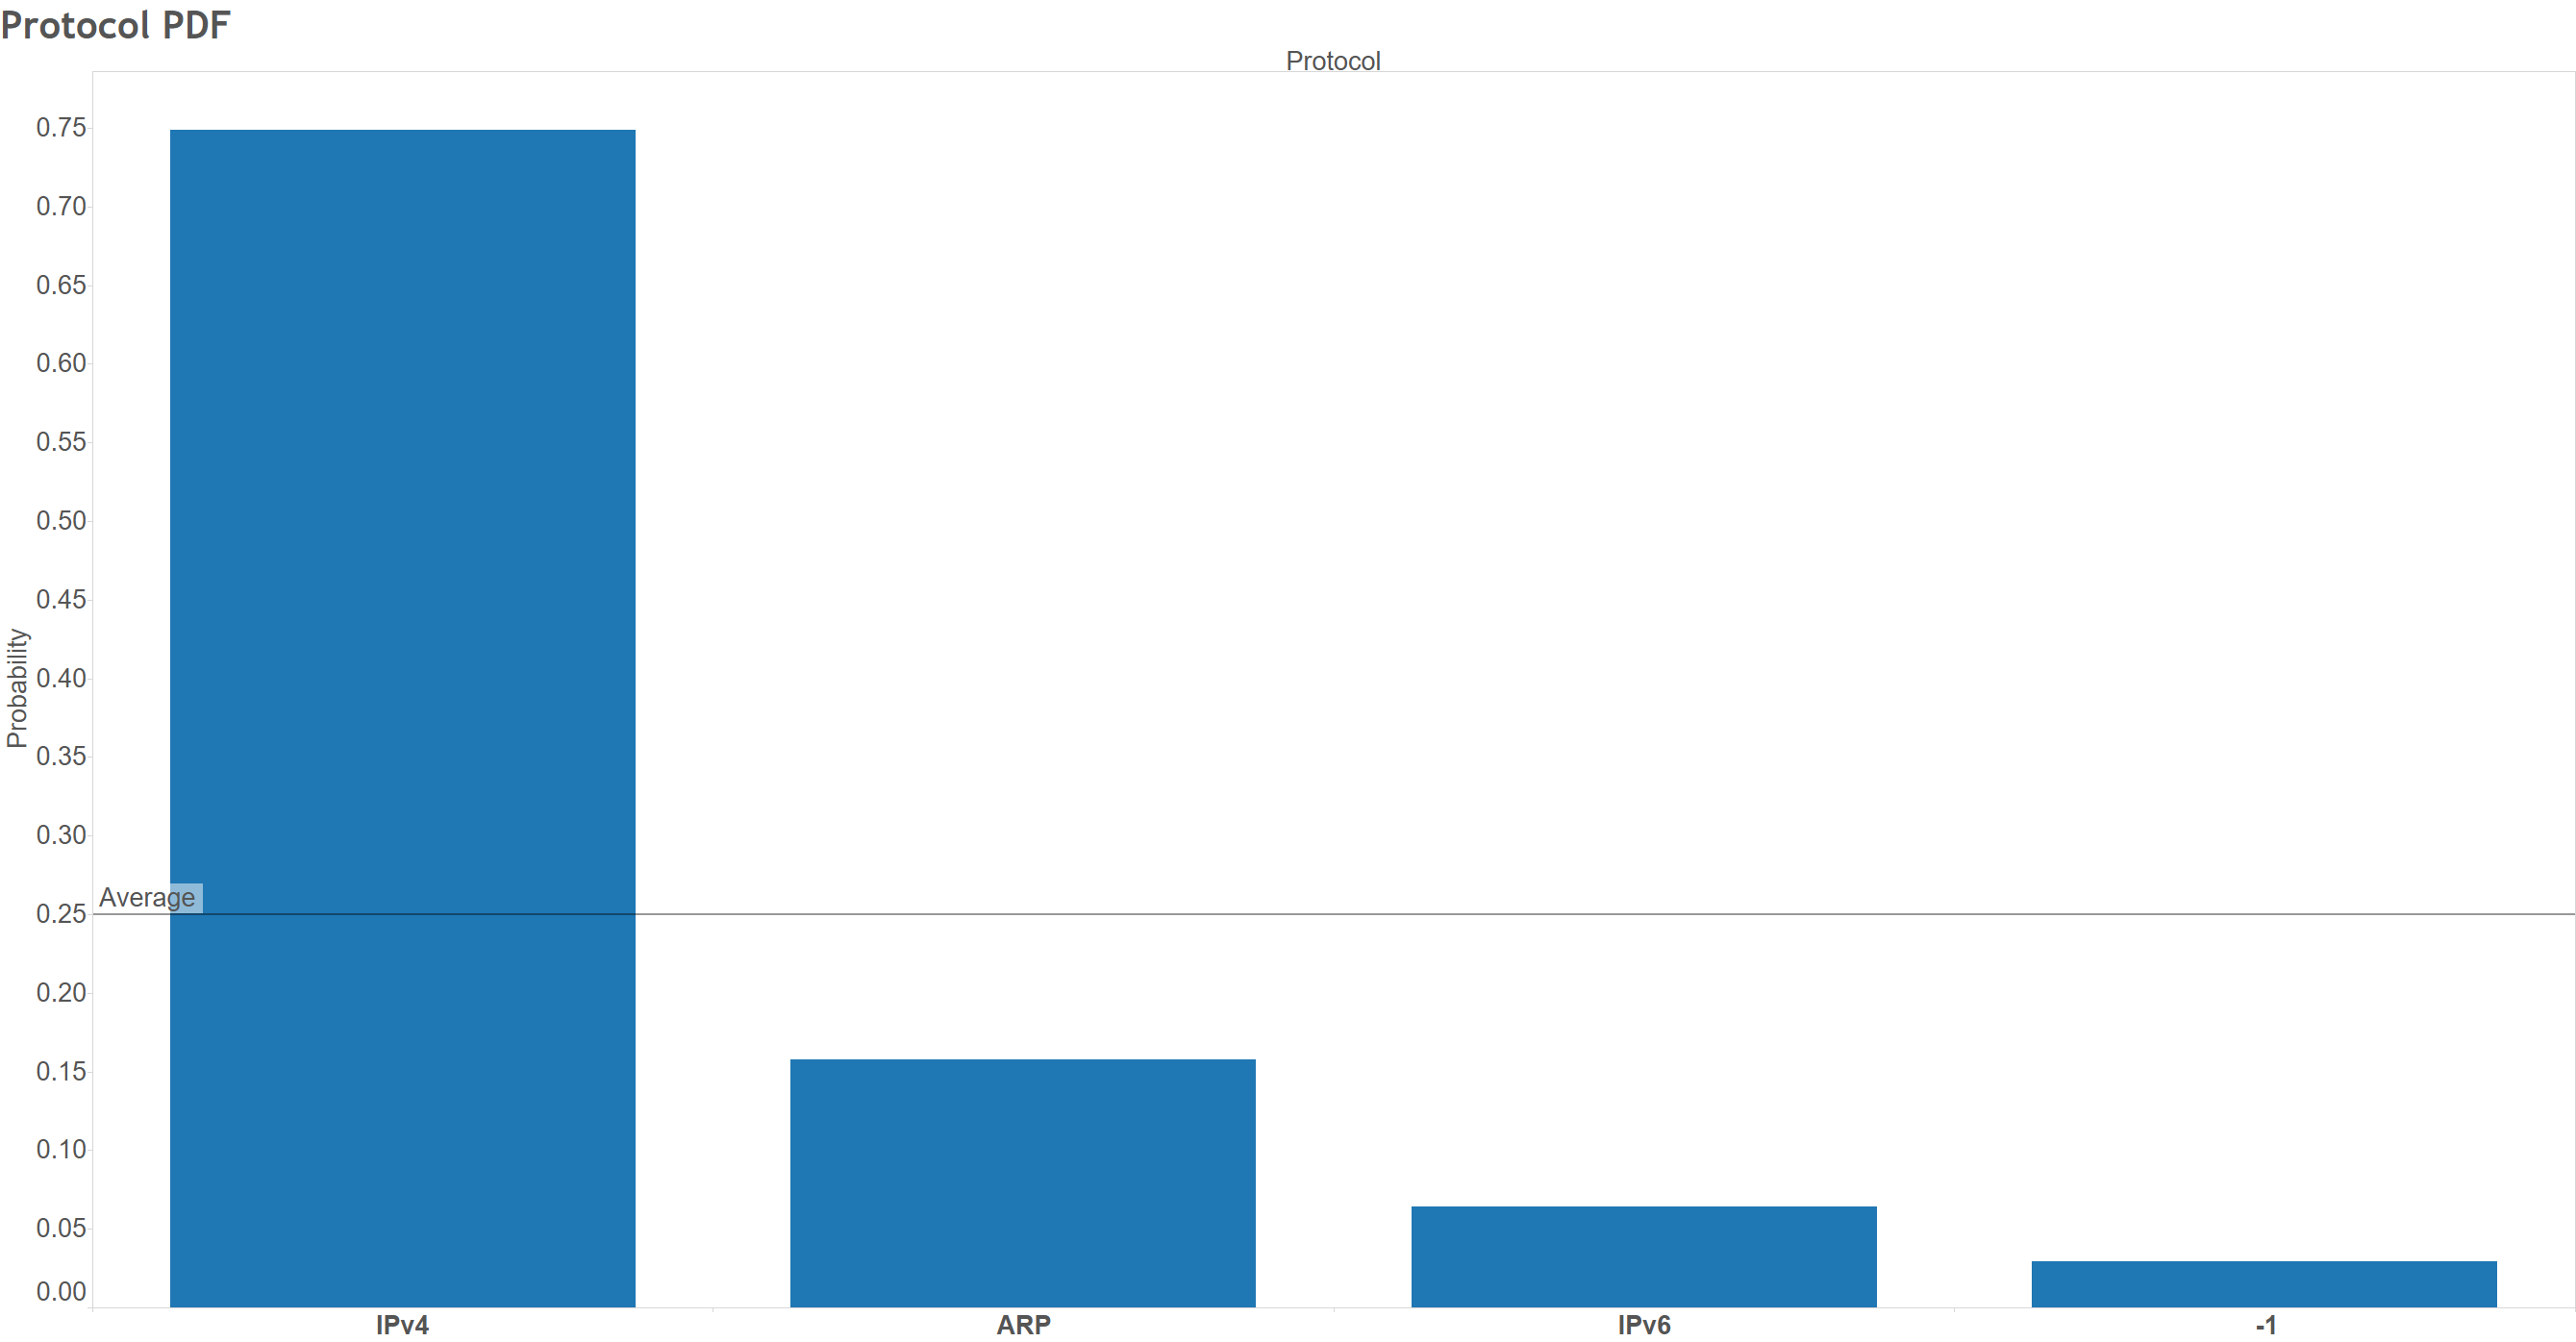
\includegraphics[width=450pt]{captures/LabosDC/Protocol PDF Dashboard Probabilitidad.png}
\caption{Probabilidad/Grado de incidencia de cada tipo de protocolo, -1 representa protocolos distintos a IPv4, IPv6 y a ARP.}
\end{figure}

Como habíamos supuesto, IPv4, ARP e IPv6 son los tres protocolos con mayor grado de incidencia en la red, esto deja en claro que los protocolo mas usados son estos 3. Algo completamente esperable, dado que:

\begin{itemize}
 
\item ARP es uno de los más necesarios para el funcionamiento de un nodo en una red de este nivel, tanto para actualizaciones periódicas de información pertinente a la red como para obtener la información esencial al momento de conectarse e iniciar las comunicaciones en dicha red.

\item IPv4 e IPv6 son los dos protocolos de transimisión de información más utilizados actualmente en computadoras personales y smartphones, que son la clase de dispositivos que es esperable encontrar con mayor frecuencia en una red del tipo de Laboratorios-DC.

\end{itemize}

Ahora podemos sacar de los datos anteriores un gráfico más estrechamente relacionado a la Teoría de la Información, si consideramos a toda la red una fuente y a cada emisión con un protocolo distinto un símbolo distinto, entonces obtenemos la siguiente figura:

\begin{figure}[H]
\centering
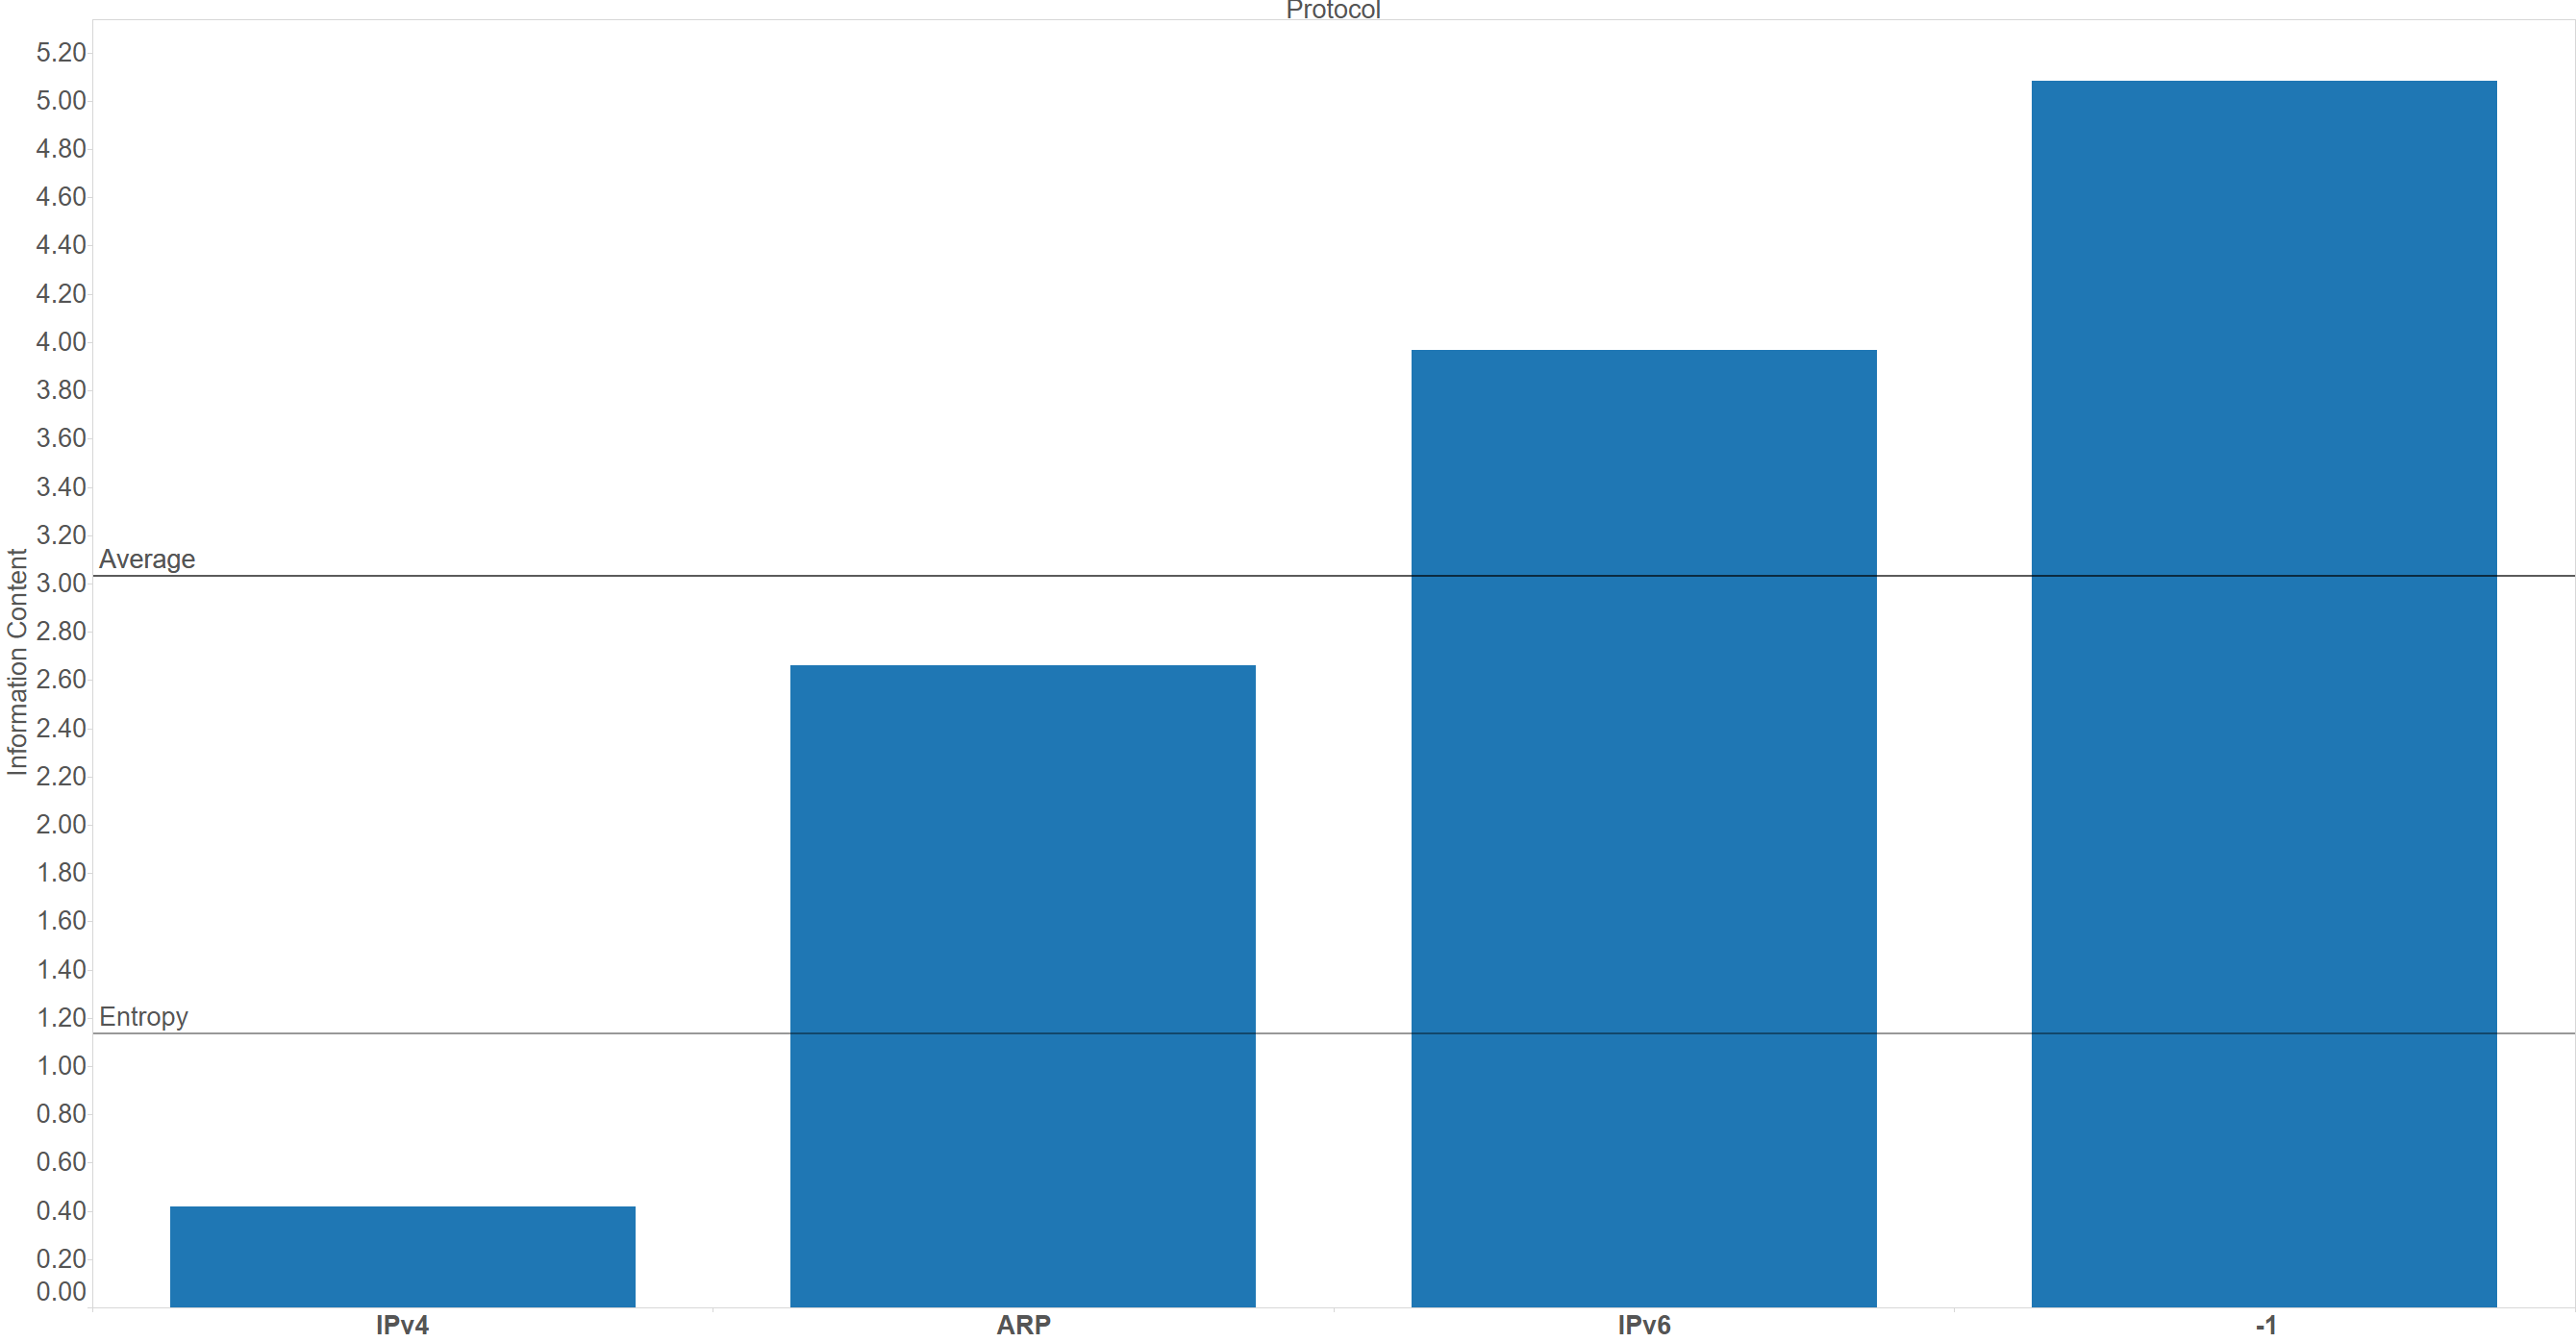
\includegraphics[width=450pt]{captures/LabosDC/Protocol PDF Dashboard.png}
\caption{Cantidad de información obtenida de un paquete de cada tipo de protocolo, -1 representa protocolos distintos a IPv4, IPv6 y a ARP.}
\end{figure}

Evidentemente, al ser más común hallar mensajes de protocolo IPv4, obtendremos menor información de esta clase de mensajes, por otro lado ARP e IPv6 se alejan más de la entropía por su menor incidencia, las apariciones del resto de los protocolos son aún menos frecuentes, por lo que obtendremos una mayor cantidad de información para estos que para cualquier otro.

Podríamos considerar un protocolo distinguido a Ipv4, debido a que es el menor (dentro de los 3 que nos interesan) en relación a la cantidad de información que proporciona, es además es más alejado dela entropía (por debajo), en este caso es alejado en el sentido de que recibiríamos una cantidad menor de información de dicha ocurrencia debido a que la ocurrencia de un mensaje de protocolo Ipv4 es relativamente común.

\subsubsection{Nodos ARP}

Ahora, pasaremos a analizar de forma más detallada los mensajes de protocolo ARP.

Podemos verlo primero observando una especie de grafo que nos permita representar de forma (muy) general las comunicaciones entre diversos nodos.

%\begin{figure}[H]
%\centering
%\includegraphics[width=450pt]{captures/LabosDC/PDFs Dashboard Probabilitidad.png}
%\caption{Comunicaciones entre IP addresses.}
%\end{figure}

\begin{figure}[H]
\centering
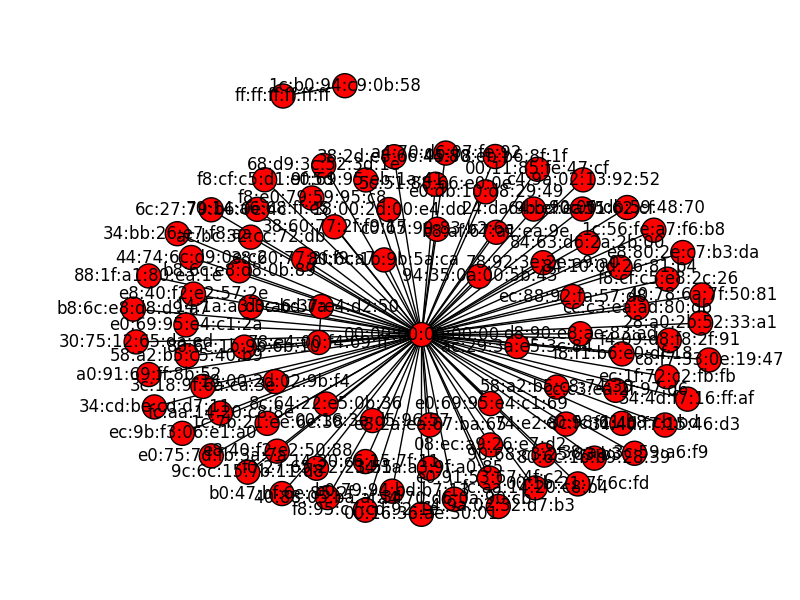
\includegraphics[width=450pt]{captures/LabosDC/conn_mac.png}
\caption{Comunicaciones entre MAC addresses.}
\end{figure}

Veamos primero algunas direcciones cuyas ocurrencias sean mayores que el resto.

Se hace evidente que existe una conexión especialmente importante con 00:00:00:00:00:00, esto quiere decir que la gran mayoría de los nodos están broadcasteando mensajes, probablemente con la intención de encontrar la MAC adress de alguna IP en particular, (que no sería extraño que fuera la perteneciente al Gateway que provee conexión con Internet, y estas suelen las conexiones mas comunes).

\begin{figure}[H]
\centering
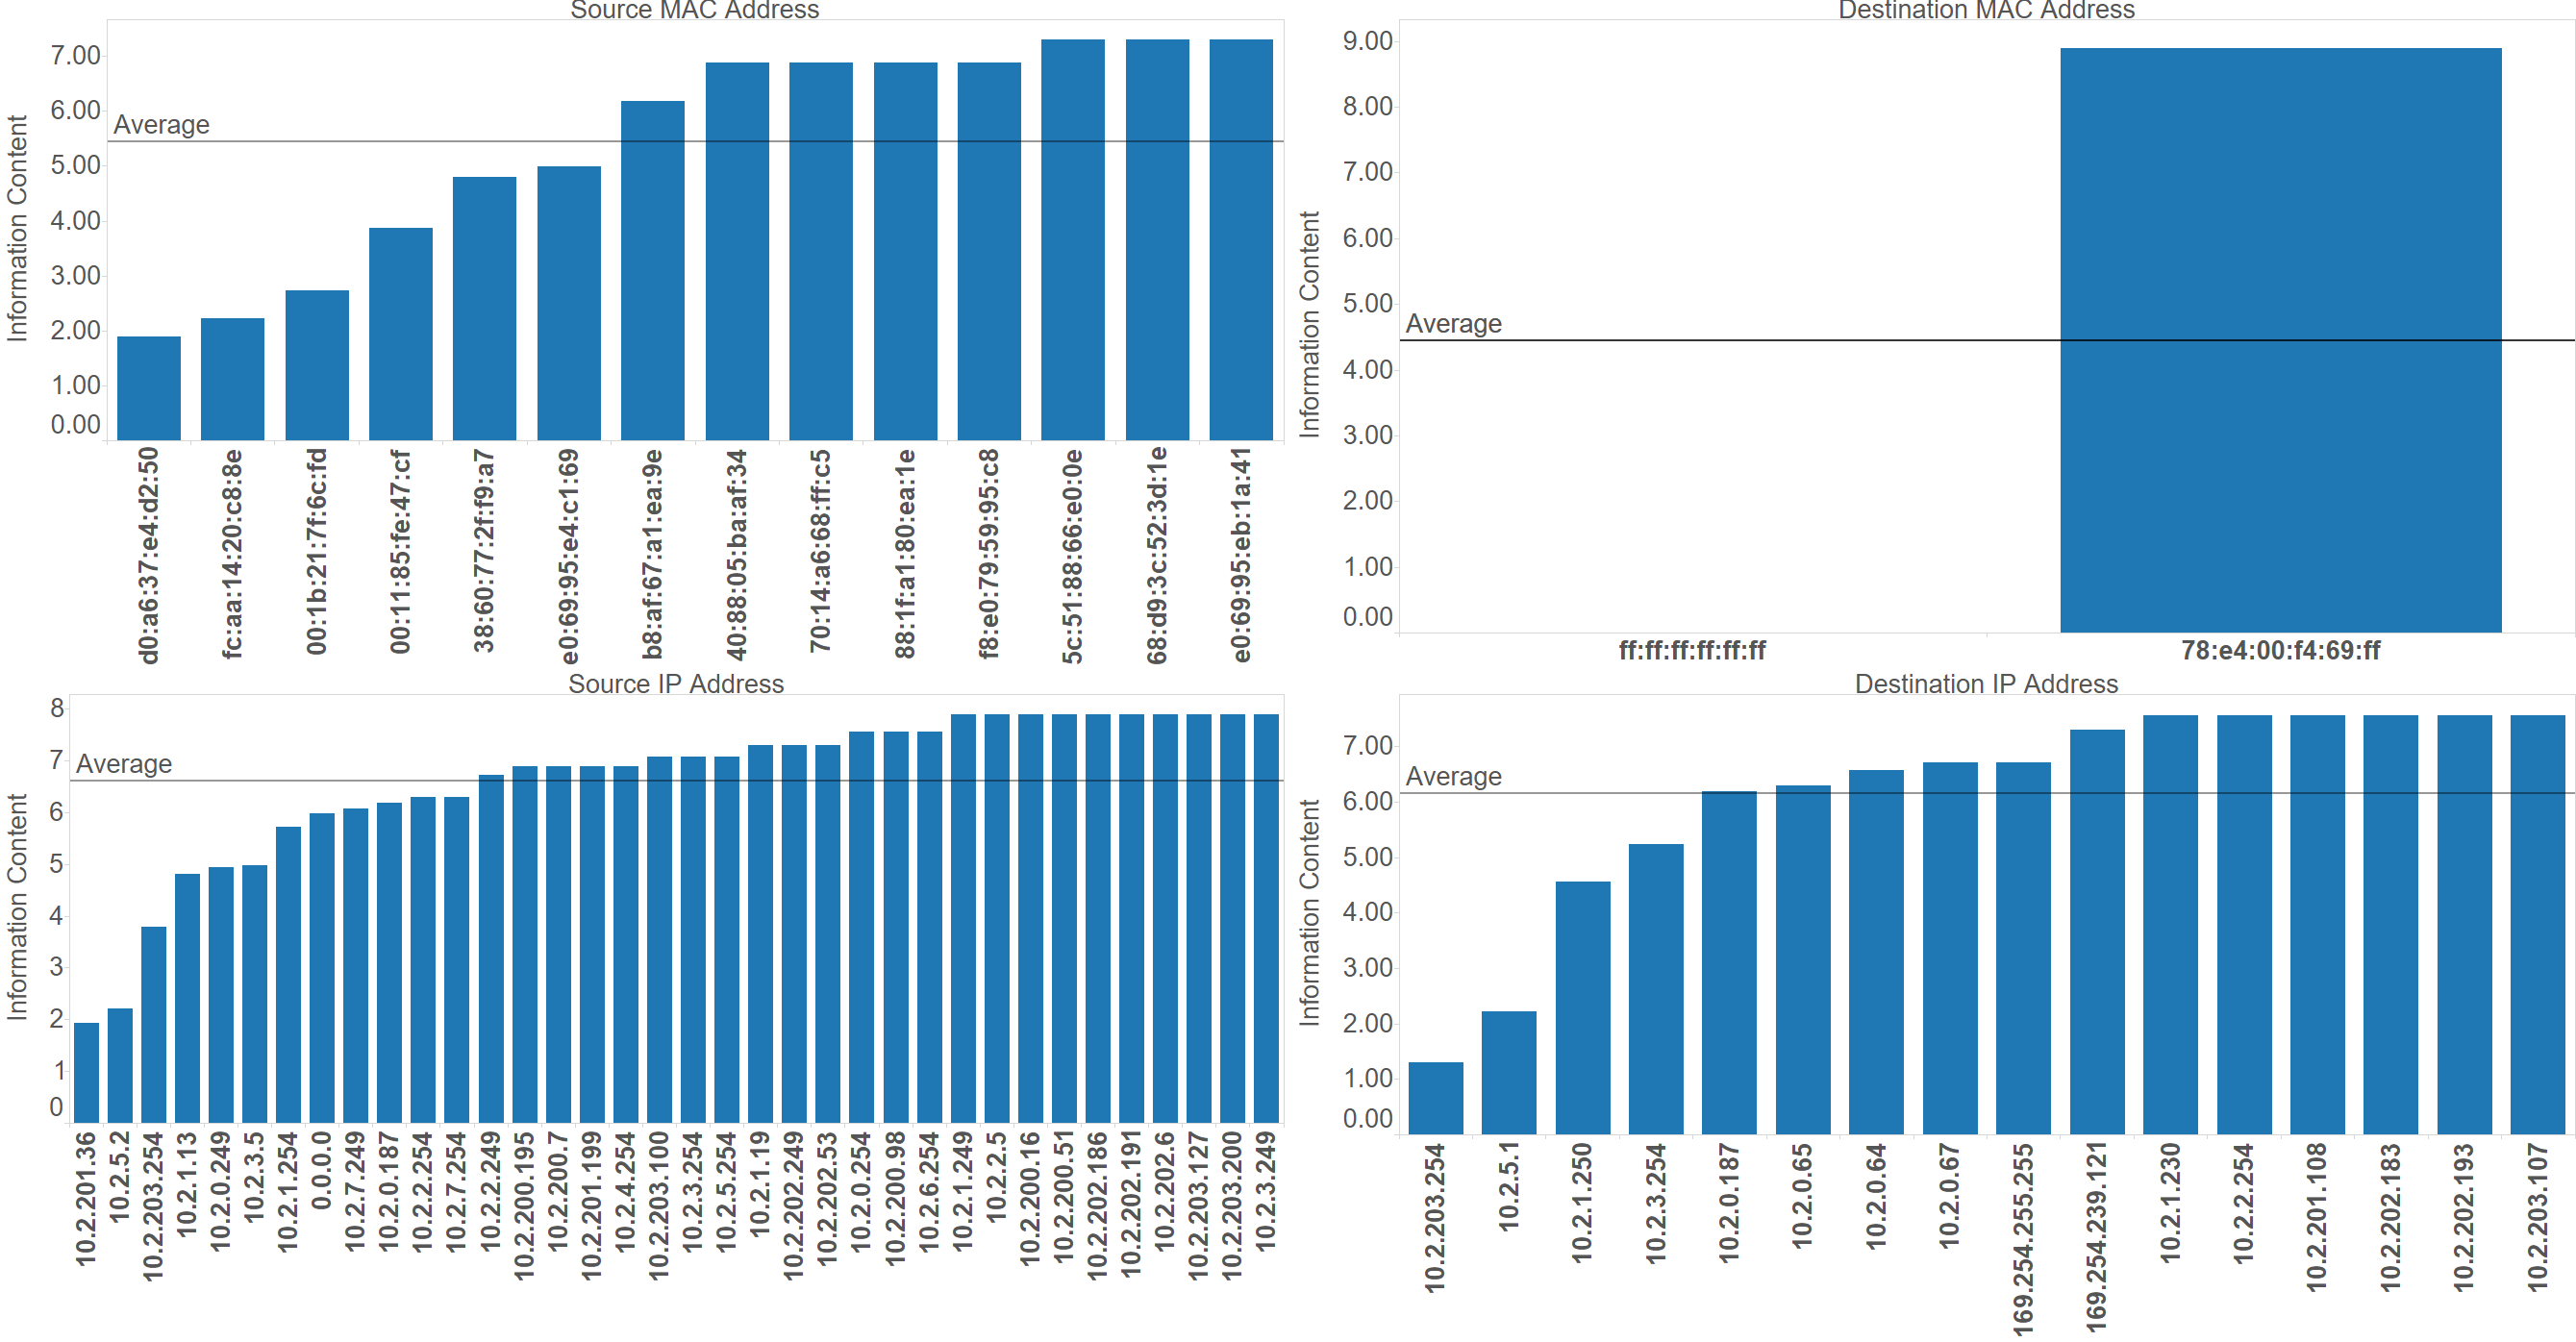
\includegraphics[width=450pt]{captures/LabosDC/PDFs Dashboard.png}
\caption{Información/Grado de incidencia de cada address, filtrando y dejando solo las address que menos informacion provean, es decir aquellas que más aparecen.}
\end{figure}

En estos graficos podemos sacarlas siguientes observaciones:

\begin{itemize}
 
\item En \textbf{Source MAC Address} no parece notarse ninguna diferencia particular entre los nodos más activos.

\item En \textbf{Destination MAC Address} se hace evidente una confirmación de lo que se había notado en el grafo visto anteriormente de direcciones MAC, la operación con más incidencia es el broadcast, en particular whois, que suelen ser algunas de las operaciones mas comunes.

\item En \textbf{Source IP Address} tampoco está tan clara una gran diferencia entre los nodos de mayor incidencia (o menor información), pero recordemos que para determinar el nodo distinguido vamos a tener en cuenta su incidencia en \textbf{Destination IP Address}.

\item En \textbf{Destination IP Address} podemos, efectivamente, determinar finalmente un nodo distinguido, el que se identifica por 10.2.203.254, que tiene mayor incidencia en destination (es el que más mensajes ARP recibe) y bastante incidencia tiene en source (es uno de los que más mensajes envían). 

\end{itemize}

En definitiva, consideramos como nodo distinguido el nodo 10.2.203.254 porque es el que más incidencia tiene en las comunicaciones del protocolo ARP de la red elegida, en particular aparece más veces en \textbf{Destination IP Adress}, por lo tanto es el símbolo que menor información provee respecto de todos los otros.

\newpage

\section{Segundo Experimento: McDonalds}

\subsection{Presentación y Suposiciones}

En este experimento, se analizó la red wi-fi de un local de McDonalds, recibimos los mensajes circulando por la red durante 20 minutos (omitimos los grafos del tráfico ARP porque es tan denso que no va a aportar información útil), procediendo luego a quedarnos sólo con los datos relevantes para el enfoque que deseamos darle a nuestro experimento.

Dividimos este experimento en dos partes principales: el análisis de los diversos protocolos existentes en la red aplicando el criterio de distinción y luego nos concentramos más específicamente en los paquetes ARP.
\subsection{Resultados}

\subsubsection{Distinción de protocolos}

\begin{figure}[H]
\centering
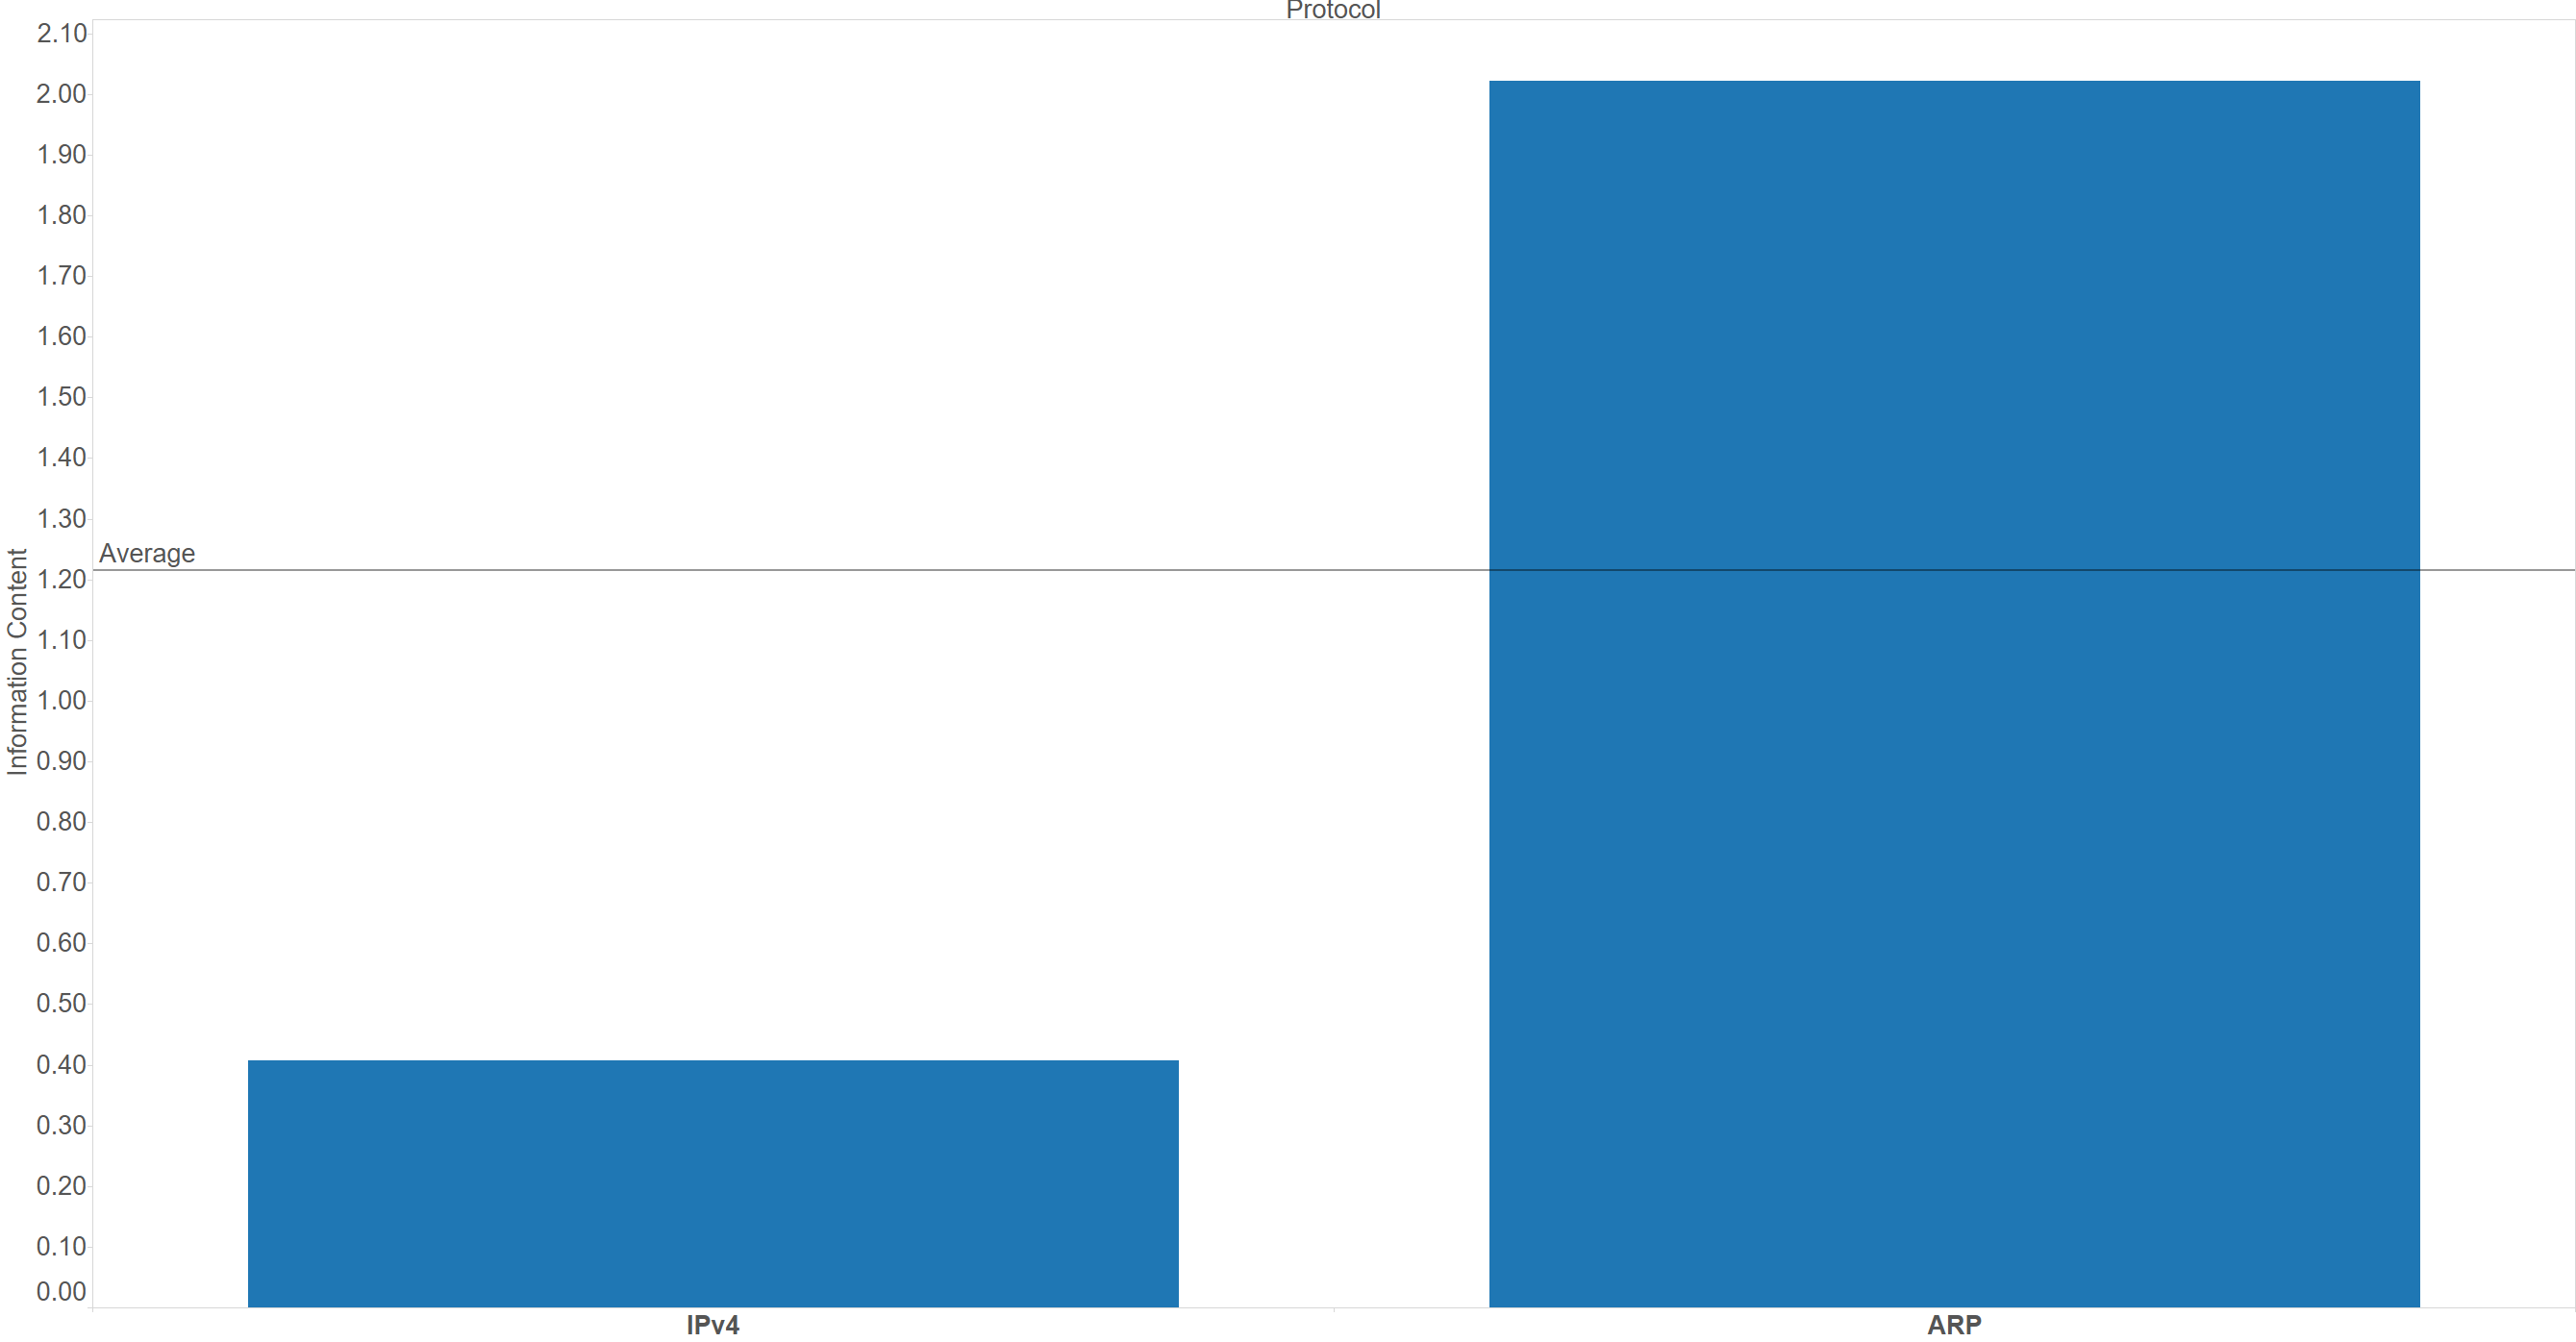
\includegraphics[width=450pt]{captures/McDonalds/20min/Protocol PDF Dashboard.png}
\caption{Información/Grado de incidencia de cada tipo de protocolo, se filtraron los protocolos con una incidencia despreciable.}
\end{figure}

Como se puede ver en el gráfico presentado, las incidencias de protocolos en cantidades no consideradas despreciables fueron de ARP e IPv4. 

Al aplicar el criterio acordado, el protocolo distinguido es IPv4, ya que es aquél que menos información provee, y es por lo tanto aquél que más alejado por debajo estuvo de la línea de la entropía.

\subsubsection{Distinción de nodos}
\begin{figure}[H]
\centering
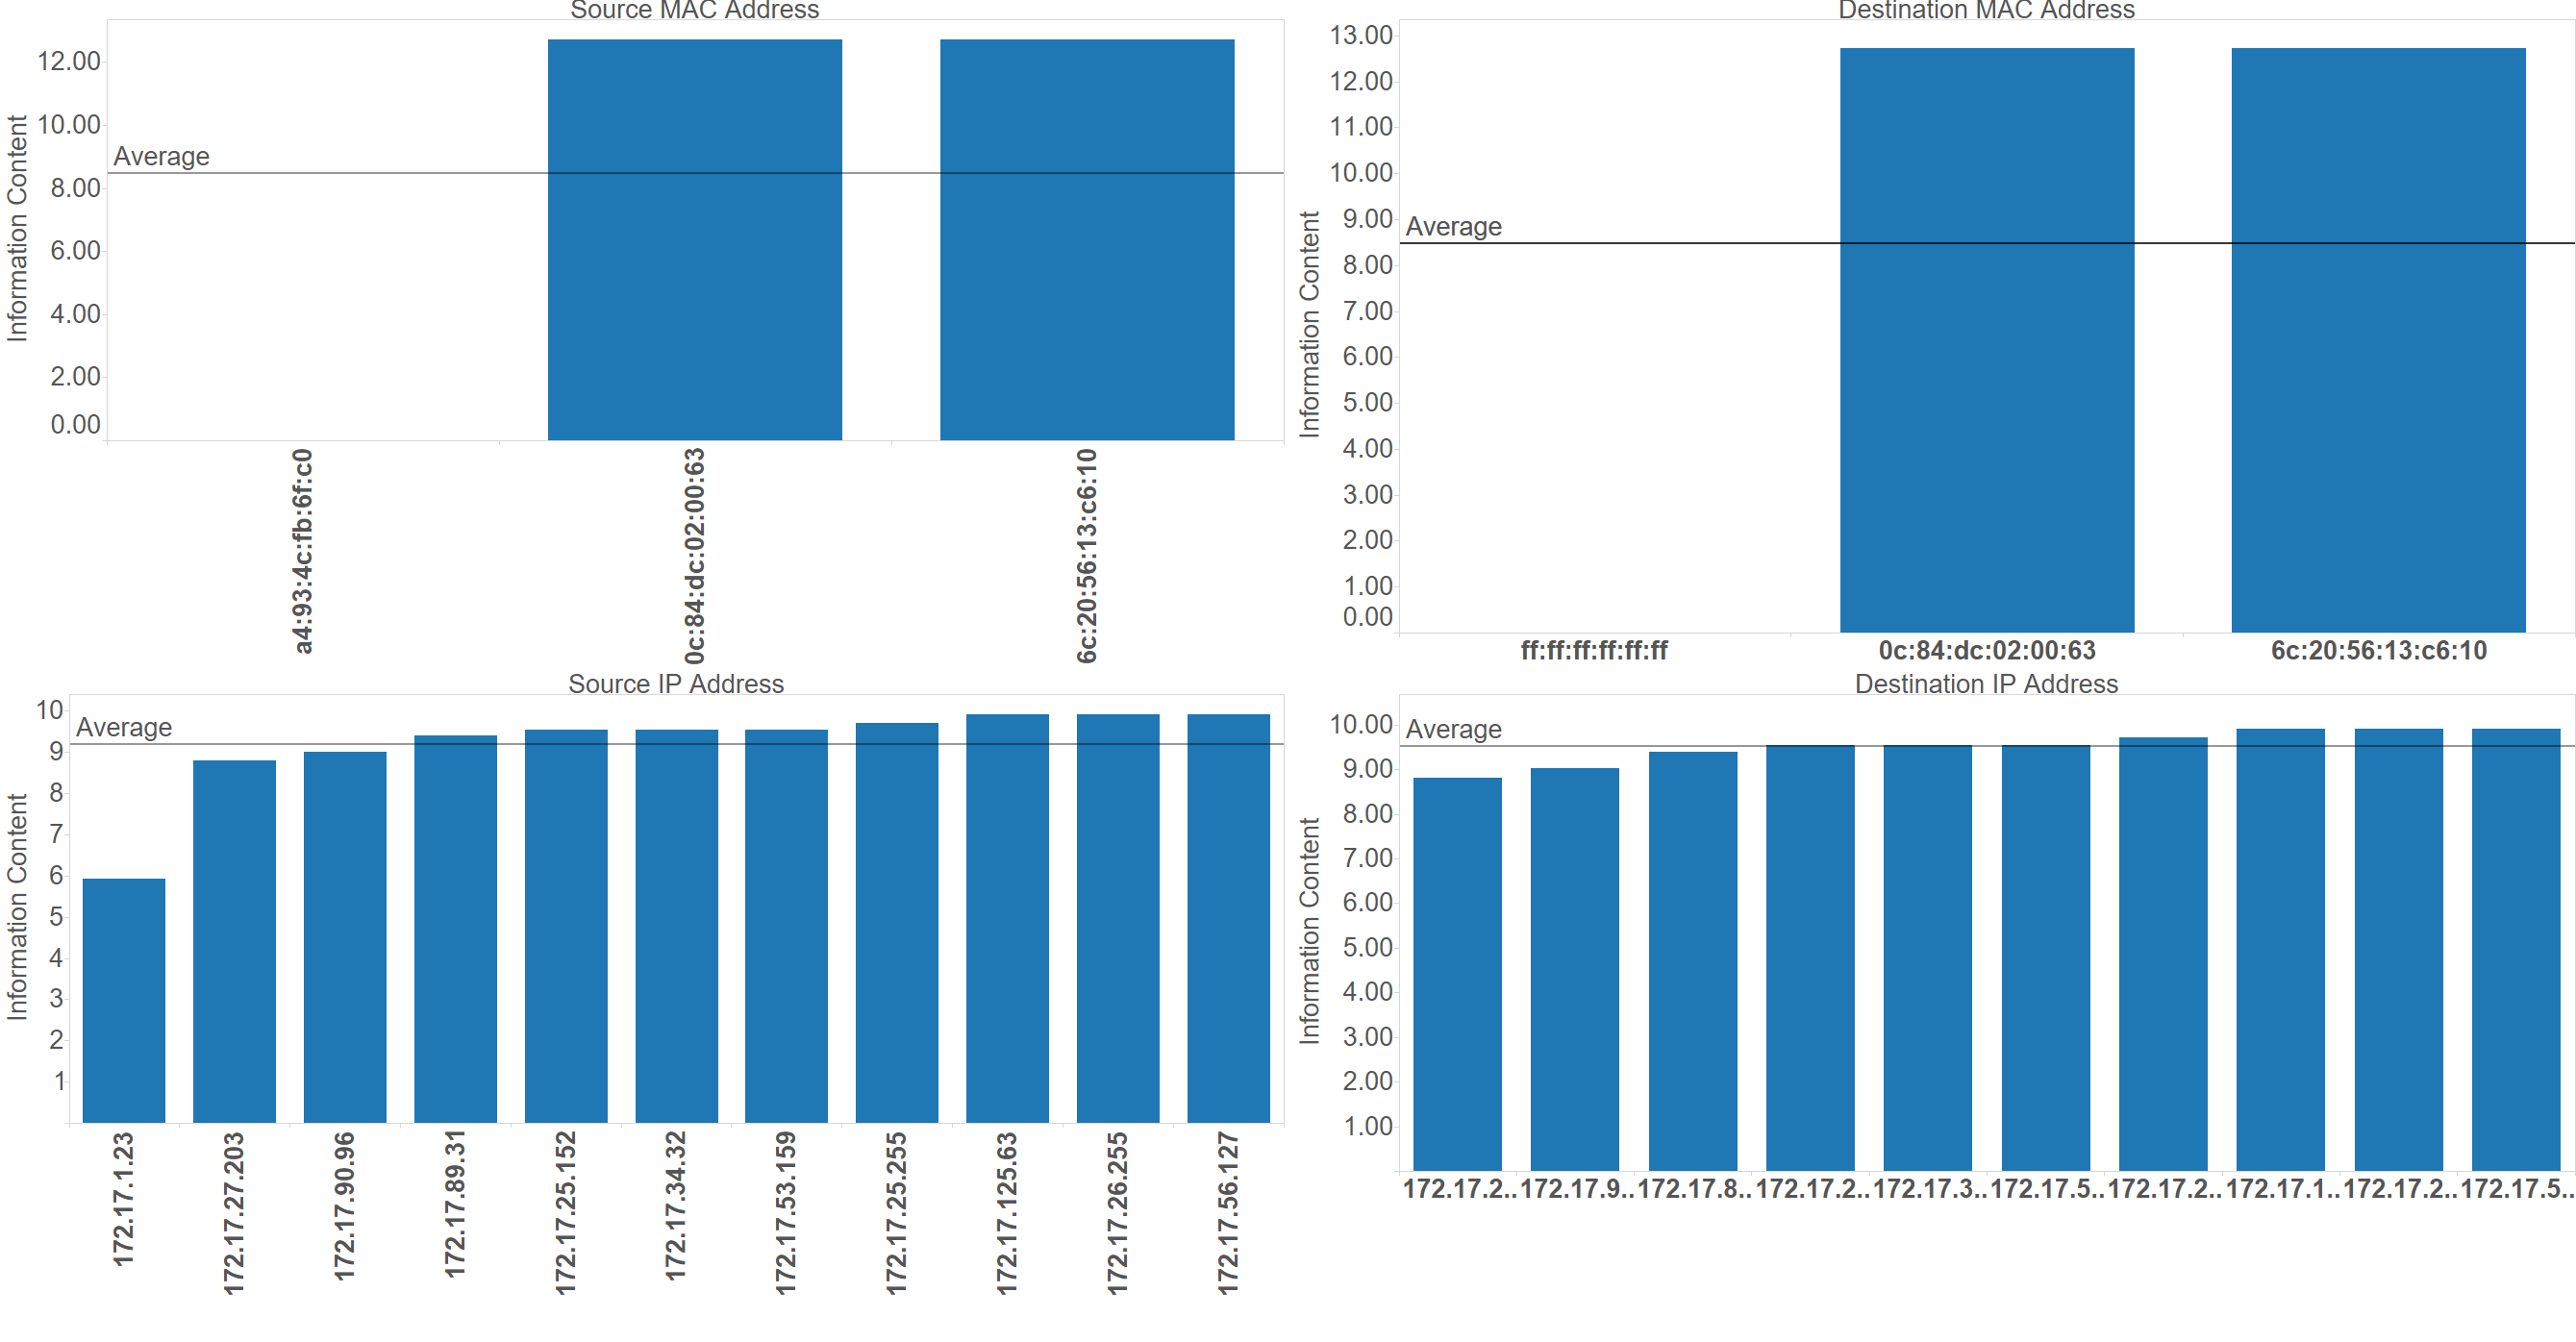
\includegraphics[width=450pt]{captures/McDonalds/20min/PDFs Dashboard.png}
\caption{Información/Grado de incidencia de source Mac Addresses, destination Mac Addresses, source IPs y destination IPs.}
\end{figure}

Estos cuatro gráficos tienen varias particularidades valiosas de analizar. Lo primero que podemos observar que nos puede llamar la atención es que los valores de la entropía son muy bajos en los primeros dos y muy altos en los otros dos. 

Es importante aclarar primero que en estos cuatro gráficos hay muchos nodos (IP o Mac Addresses depediendo del gráfico) que no aparecen debido a que su probabilidad es tan baja que decidimos no incluirlos. Una de las razones por las cuales puede ocurrir esto es que se trataba de una red sin ninguna clave y un dispositivo podía conectarse y desconectarse inmediatamente, porque por ejemplo pertenecía a alguna persona que pasaba por ahí. Este puede ser uno de los motivos por los cuales hay tantos nodos que aportan una cantidad de información similar. Entonces la entropía es tan alta en los segundos casos porque toma en cuenta la información promedio de \textbf{todos} los nodos, incluso aquellos que decidimos sacar. 


En el caso de los dos primeros gráficos la entropía es tan baja debido a la gran diferencia en la información que aportan la primer Mac Address con respecto a las demás. El promedio en cambio, es bastante más alto ya que hay más Mac Addresses (tanto source como destination) que aportan más información que la primera.


El nodo distinguido, siguiendo el mismo criterio de tomar la Destination IP con menor información en este caso es 172.17.1.23.

\subsubsection{Relación IP Address - MAC Adrress}
\begin{figure}[H]
    \centering
    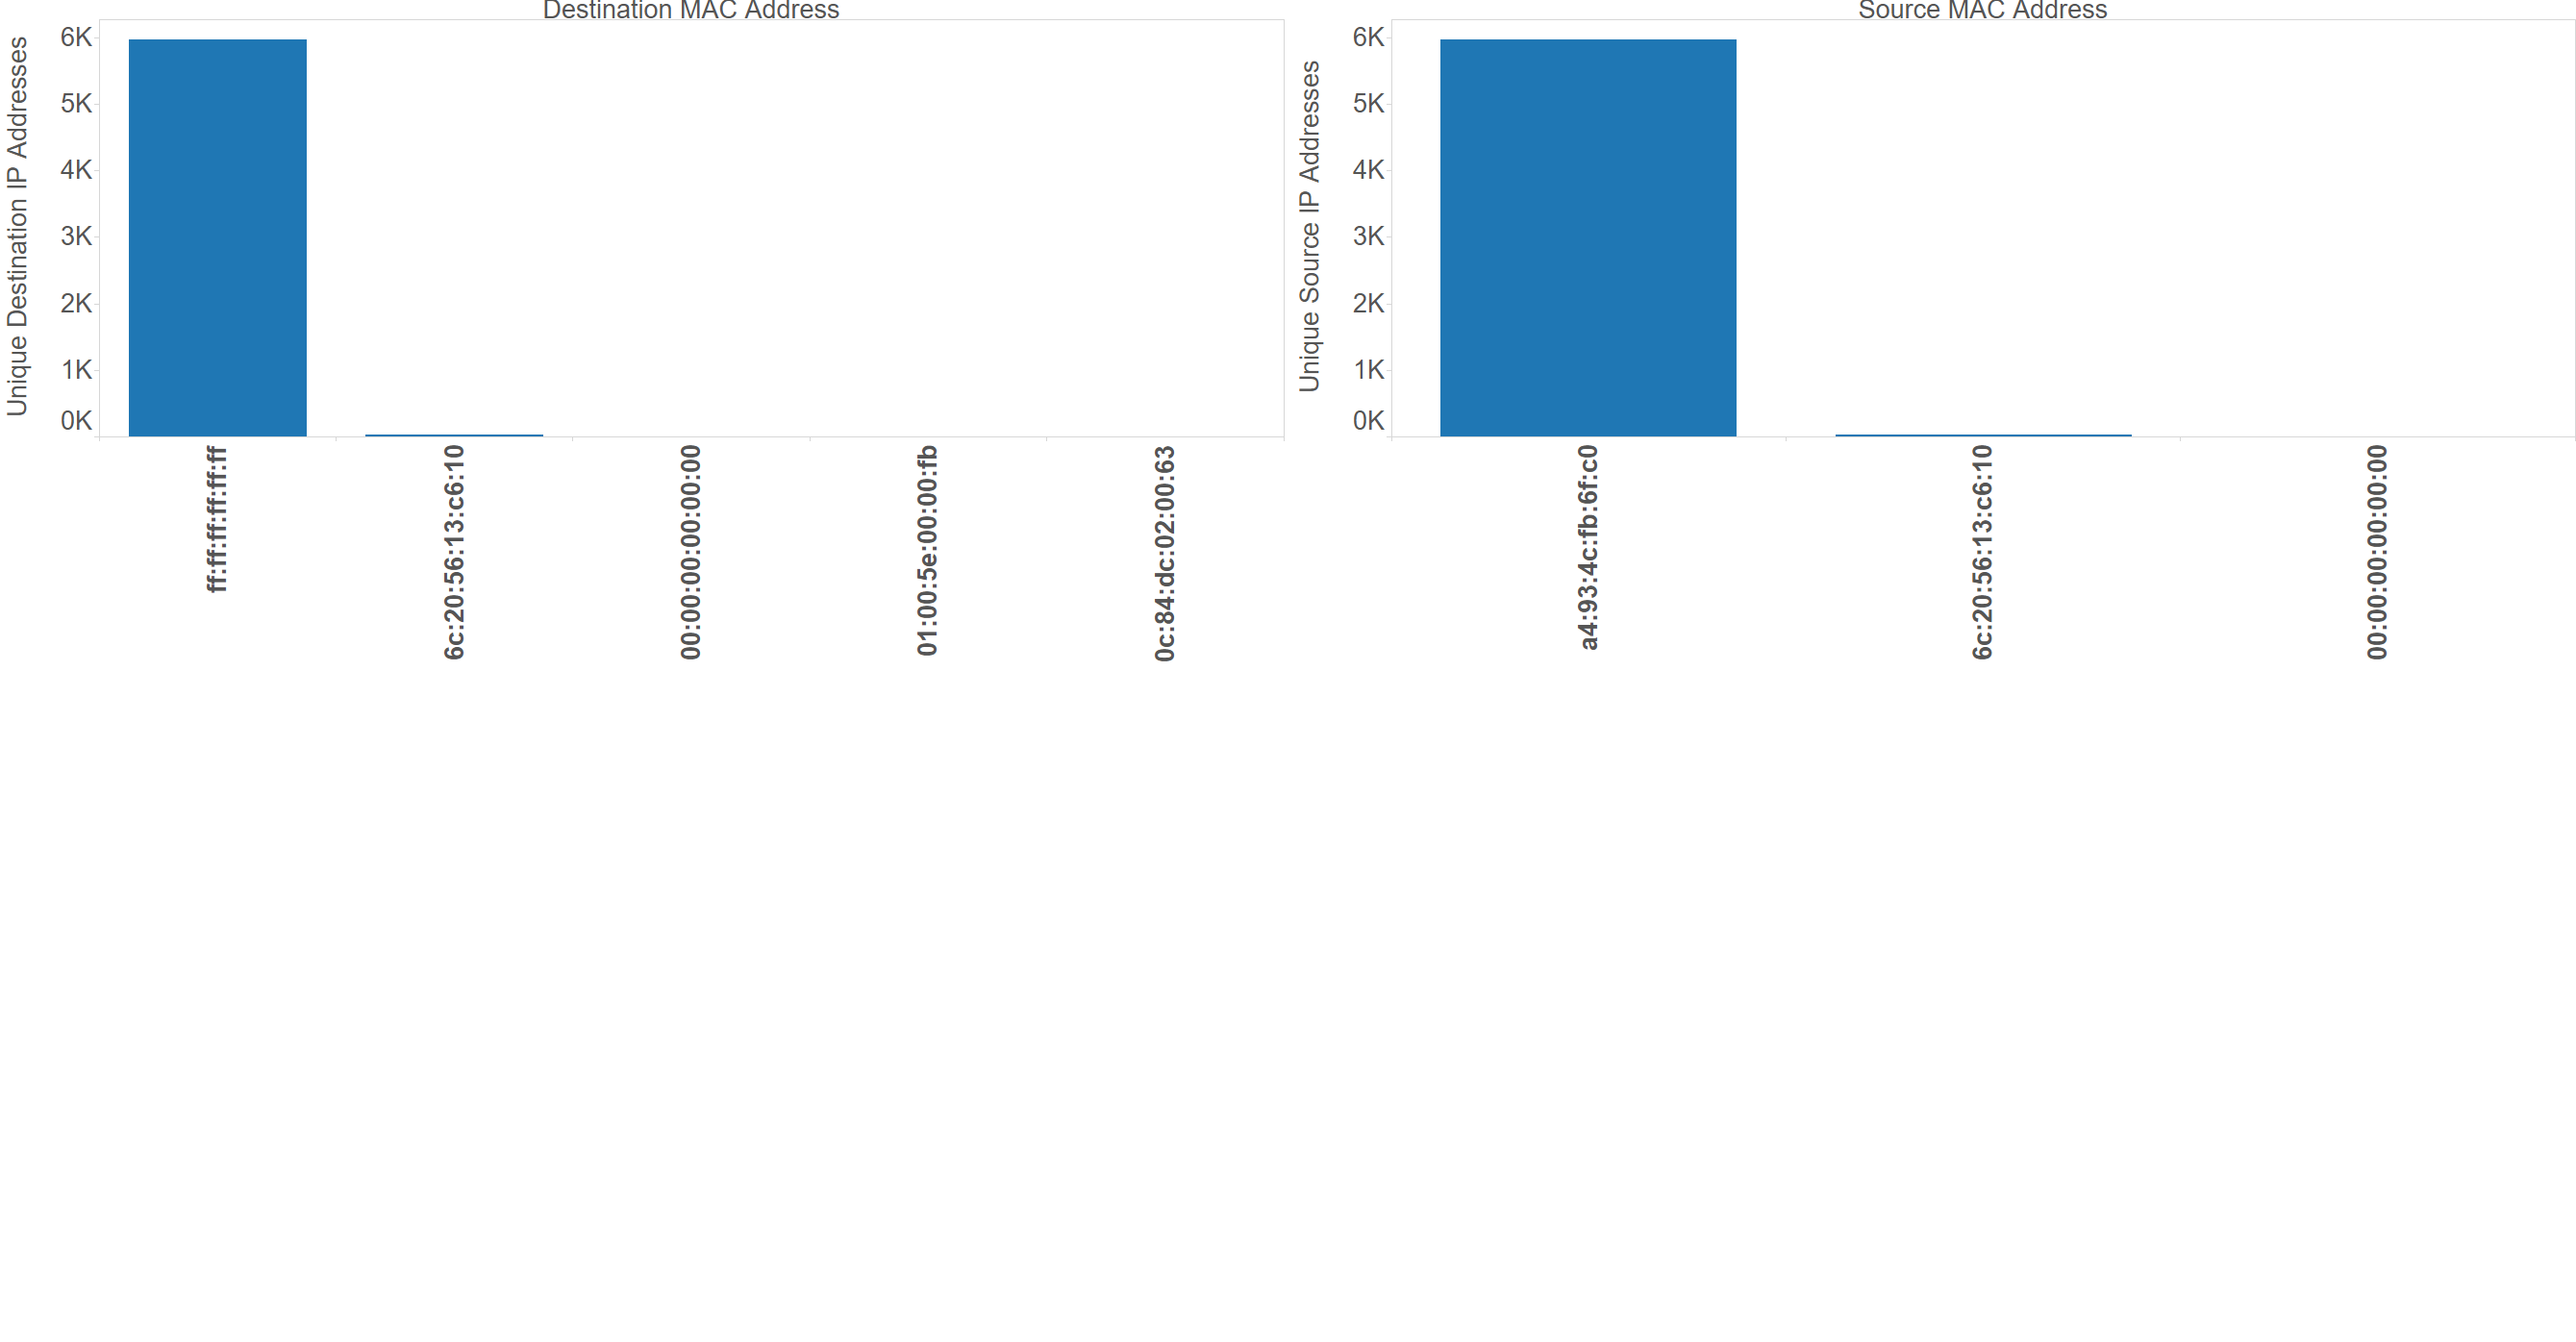
\includegraphics[width=1\textwidth]{captures/McDonalds/20min/IP vs MAC Correspondence.png}
    \caption{Estos cuatro gráficos nos dan información sobre la relación entre las IP y Mac Addresses.}
    \label{fig:mesh1}
\end{figure}


\newpage

\section{Tercer Experimento: Red Laboral}

\subsection{Presentación}
Para este experimento se analizo una red laboral bastante grande de una empresa de servicios web (MercadoLibre), con una infraestructura de red compleja. 
El tiempo de captura fue de 20 minutos aproximadamente, en el cual se logro capturar alrededor de 160000 paquetes. De los cuales 15000 fueron IP, 2700 ARP, 3500 IPv6 y solo 2 paquetes contenían protocolos desconocidos.
Hubo una peculiaridad en esta captura, no se capturo ni un ARP is-at, se uso la misma computadora y el mismo script para capturar. De hecho después analice la misma red directamente con wireshark y sucedió lo mismo.

\subsection{Resultados}
\subsubsection{Protocolos}
Para esta fuente de información, como dije previamente, los únicos símbolos presentes fueron 3: IPv4, IPv6 y ARP. Veamos cual es la información de cada símbolo:

Foto de protocolos

Se puede ver claramente que IPv4 presenta poca información a la fuente, esto significa que se presenta mucho en esta captura. Además veamos que los otros dos protocolos, al mostrar un contenido de información mayor, significan que no incidieron mucho en nuestra red.

Veamos las probabilidades ahora para ver mas claro el resultado a la hora de hablar de cantidades:

Imagen de probabilidades

Es claro que IPv4 fue el protocolo que mas apareció por mucho, lo cual coincide con lo que contábamos en la presentación. 

En interesante ver que, aunque en poca cantidad, se ve un trafico IPv6, por lo que uno asume que cierta infraestructura debe haberse migrado al nuevo protocolo.

\subsubsection{Nodos ARP}
En este experimento, como contamos antes, no hubo ningún trafico capturado de packetes ARP is-at. Esto nos resulto muy extraño, ya que es la base de la capa de enlace. En esta red WiFi, hay una única SSID pero varios access points, y para nosotros es una incógnita como se maneja el hecho de crear una única subnet a la que se puede acceder desde varios puntos de accesos. Por un lado suponemos que debería hacerse un broadcast a todos los AP de todo paquete broadcasteado en cualquiera de ellos, ya que un host va a buscar enviar un paquete a otro host en su subnet utilizando su dirección física y sin necesidad de ser routeado por el AP. Por otro lado, al ser una red tan grande, esto generaría mucho trafico en toda la red subneteada. Lo que terminamos suponiendo es que los paquetes no se broadcastean a todos los APs ya que en ese caso habría una mayor posibilidad de ver ARP is-ats, pero al no tener ninguno no pudimos analizar muy bien esta situación.

\newpage
\section{Cuarto Experimento: Red Controlada}
\subsection{Características y condiciones de la red}
Dado que ya analizamos tres redes con una cantidad importante de nodos y tráfico, decidimos en este experimento tratar con una red casera debido a que tenemos más control sobre la misma y podemos verificar hipótesis más fácilmente por nuestro conocimiento. Se trata de una red wifi compuesta por siete dispositivos (entre ellos tablets, celulares y computadores). Además, para aumentar las chances de tener un tráfico de paquetes ARP considerable, reseteamos el router antes de comenzar a capturar el tráfico con el objetivo de vaciar la caché que almacena el mapeo de IP's a Mac Addresses.
\par Como se trata de una red de pequeñas dimensiones, para poder hacer una captura que realmente nos brinde información valiosa para analizar necesitamos estar capturando el tráfico un tiempo mayor que en los casos anteriores. En las redes anteriores si hacíamos capturas de unos pocos segundos ya teníamos muchísimos datos por las dimensiones de las redes y por eso los tiempos de captura no superaban los 30 minutos. Es por eso que en este caso decidimos capturar el tráfico durante una hora.
\subsection{Resultados}
\subsubsection{Grafo de tráfico ARP}
\begin{figure}[H]
    \centering
    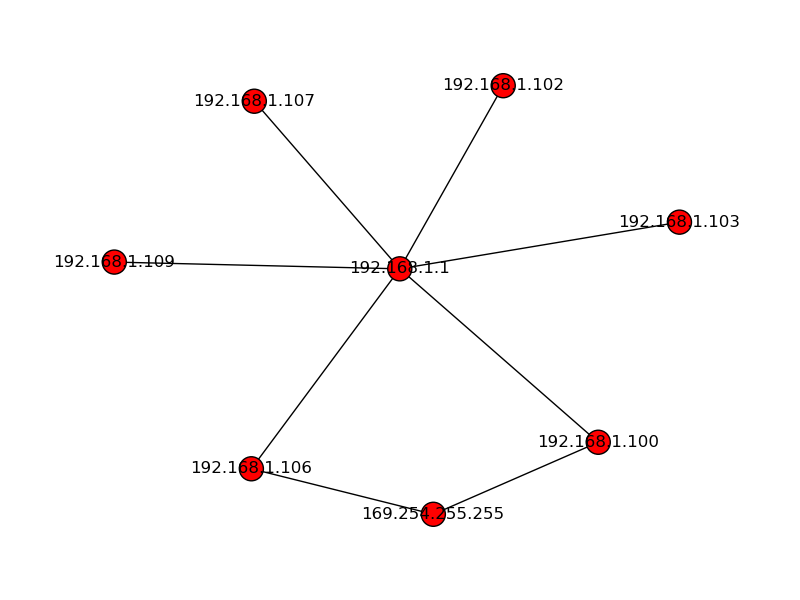
\includegraphics[width=0.70\textwidth]{../captures/CasaGerman/conn_ip.png}
    \caption{Tráfico de paquetes ARP en la red, distinguiendo nodos por IP.}
    \label{fig:mesh1}
\end{figure}
El gráfico anterior nos permite tener un panorama general de los nodos de la red según el envío de paquetes ARP. Lo primero que puede parecer extraño al observar este gráfico es que aparece una IP un tanto extraña (169.254.255.255) en comparación con las demás. Investigamos un poco sobre este tema y resulta que esta IP es asignada a un dispositivo de manera automática cuando no encuentra otra. Esto es muy común que suceda en sistemas Windows aunque también pasa en dispositivos Mac y se da cuando existe algún problema para asignar una IP al dispositivo.
\par Otra cosa que podemos ver es que el grafo tiene una forma de estrella centrada en un nodo cuya IP es 192.168.1.1, tiene sentido pensar que este nodo es el router ya que es el que se comunica mediante el protocolo ARP con todos los demás nodos (excepto el que tiene una IP distinta por motivos que ya explicamos antes). Debido a que esta es una red conocida por nosotros, pudimos efectivamente corroborar esto (comando route -n de Ubuntu) y era verdad, el nodo cuya IP es 192.168.1.1 corresponde al router.
\begin{figure}[H]
    \centering
    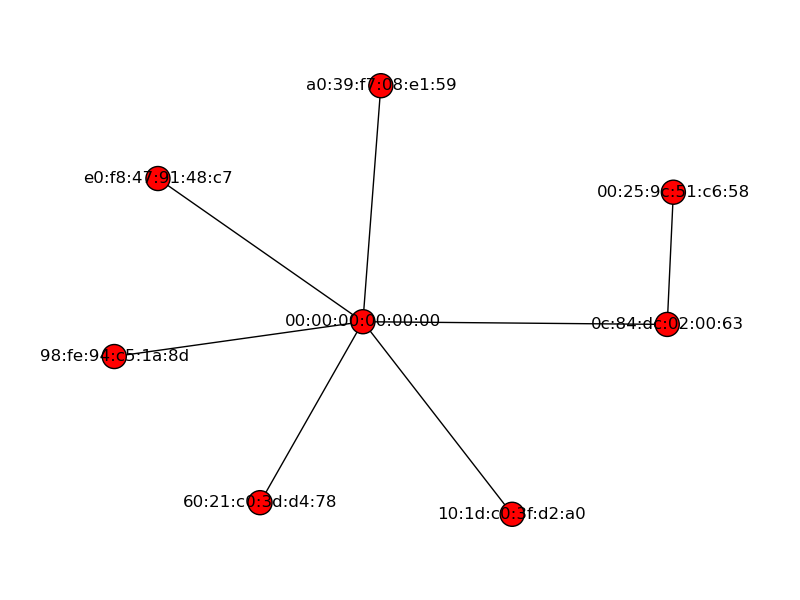
\includegraphics[width=0.70\textwidth]{../captures/CasaGerman/conn_mac.png}
    \caption{Tráfico de paquetes ARP en la red, distinguiendo nodos por Mac Address.}
    \label{fig:mesh1}
\end{figure}
Este gráfico es similar al anterior en el sentido de que nos revela el tráfico de paquetes ARP pero nos permite diferenciar a los nodos segun sus Mac Addresses.

\subsubsection{Distinción de protocolos}
\begin{figure}[H]
    \centering
    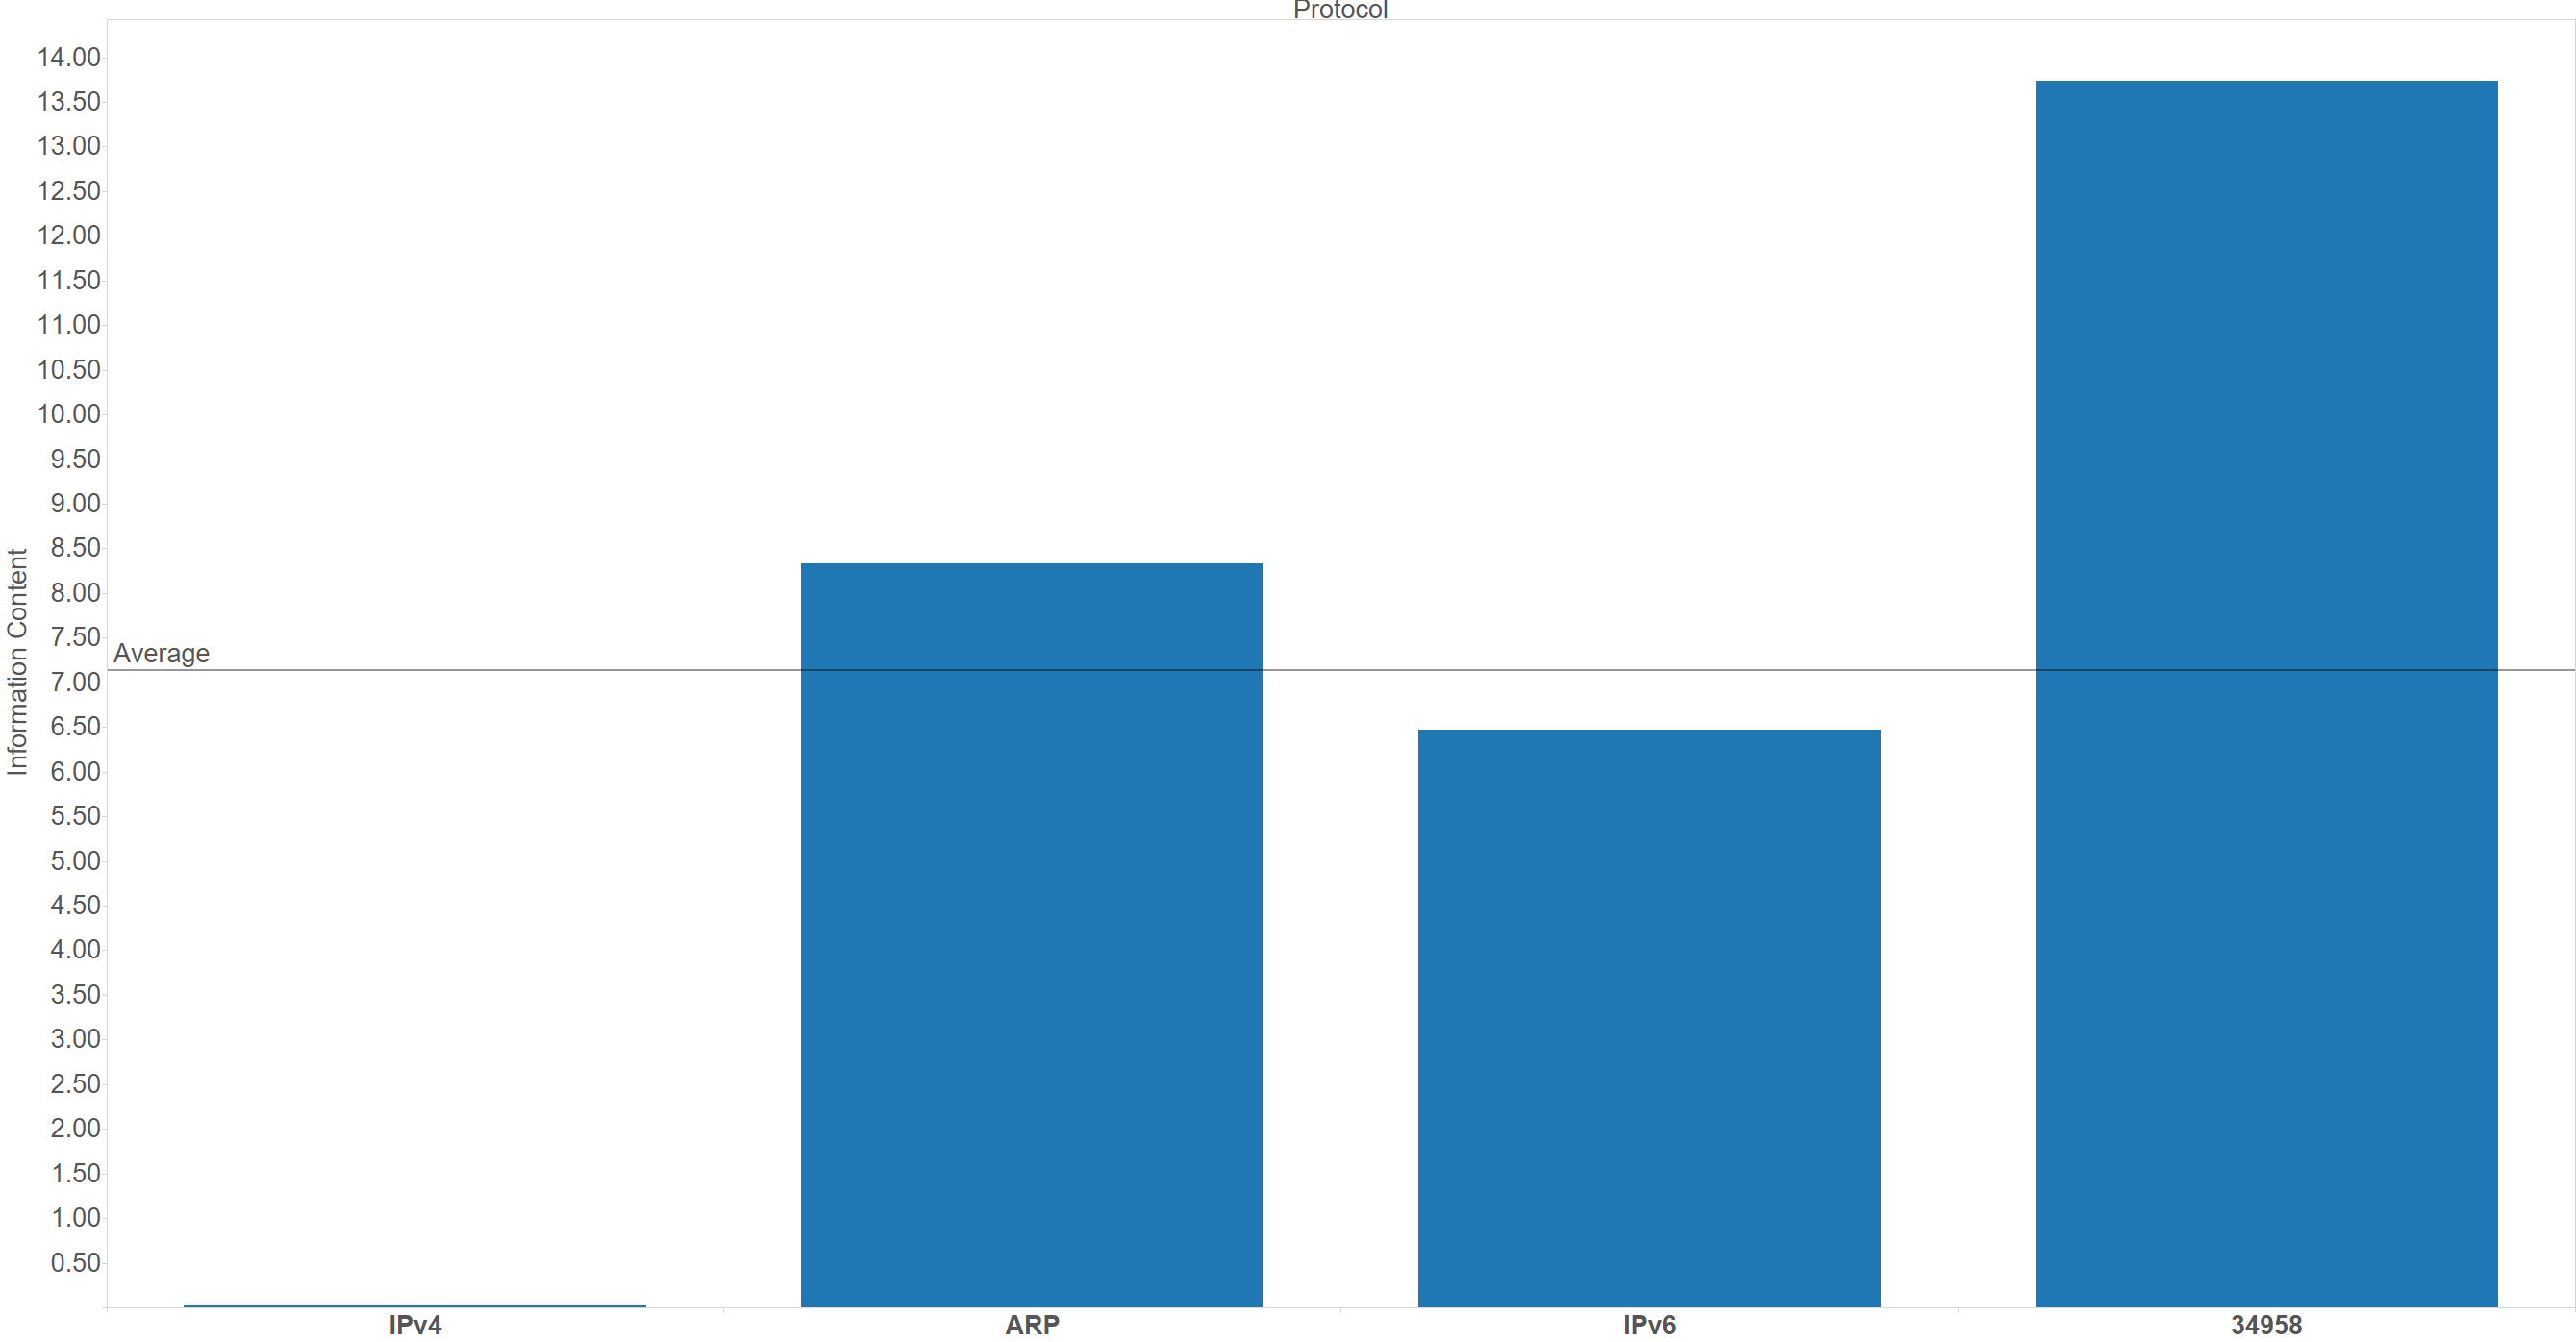
\includegraphics[width=1\textwidth]{../captures/CasaGerman/Protocol PDF Dashboard.png}
    \caption{Este gráfico nos muestra la cantidad de información que provee cada protocolo a la fuente (donde los símbolos son los protocolos), información promedio y entropía.}
    \label{fig:mesh1}
\end{figure}
Si observamos la línea que representa la entropía, vemos que se trata de un valor muy bajo, indicando que se trata de una fuente predecible en cuanto a los símbolos que emite.
\par En cuanto a los símbolos en sí, vemos que la información proveída por IPv4 es muy pequeña mientras que la del protocolo 34958 es muy alta y las correspondientes a ARP e IPv6 son alrededor de la mitad de 34958. El protocolo distinguido es claramente IPv4 ya que es el que menos información tiene y por lo tanto el más utilizado. Los otros protocolos tienen información bastante más elevada, esto se debe a que al ser una red casera el tráfico de paquetes ARP (por ejemplo) es bastante más reducido ya que la cantidad de dispositivos es reducida y es más fácil y rápido para el router llenar la caché que vincula IP Addresses con Mac Addresses.

\subsubsection{Distinción de nodos}
\begin{figure}[H]
    \centering
    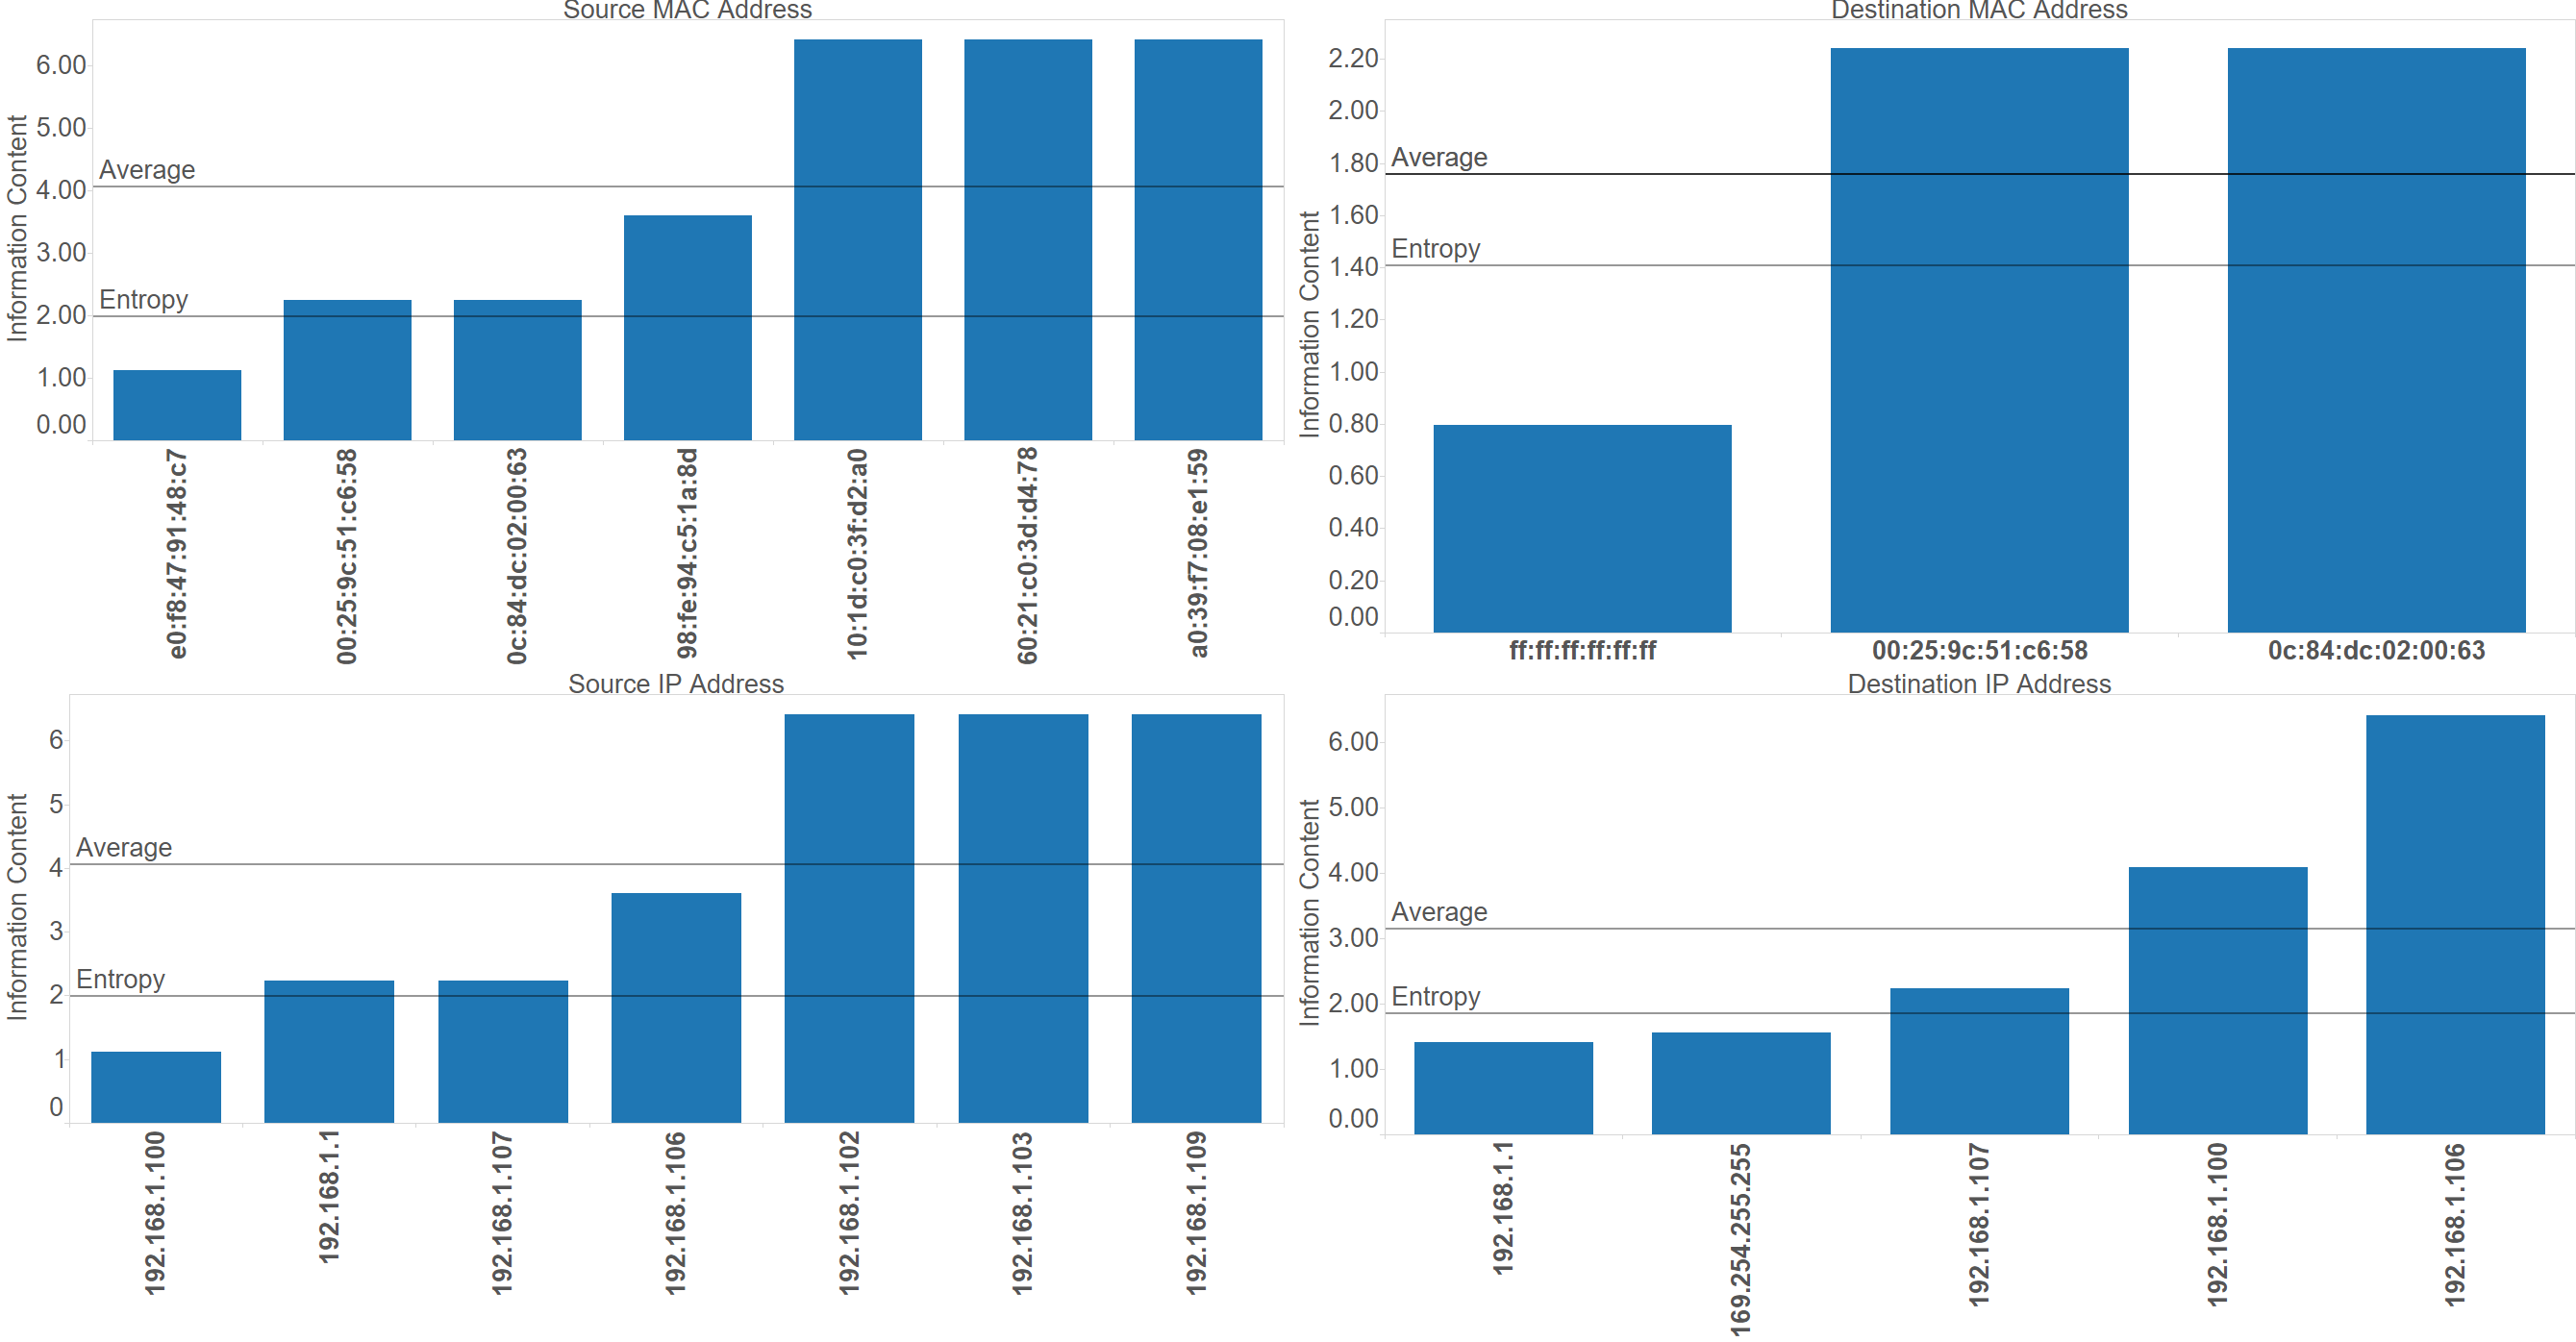
\includegraphics[width=1\textwidth]{../captures/CasaGerman/PDFs Dashboard.png}
    \caption{Al capturar paquetes ARP y quedarnos con las direcciones Mac de source como símbolos de la fuente obtenemos el gráfico de la esquina superior izquierda que nos muestra la información de cada nodo (visto como Mac Address), si nos quedamos con las Mac de destino de los paquetes obtenemos el de la derecha que nos muestra la información de cada nodo. Análogamente tenemos los gráficos de abajo que utilizan direcciones IP.}
    \label{fig:mesh1}
\end{figure}

Para poder elegir el nodo distinguido (podría ser más de uno) vamos a utilizar el gráfico de Destination IP Address y tomar la IP de destino con menor cantidad de información (respetando así el criterio fijado al principio). En este caso dicha IP es 192.168.1.1 que es la correspondiente al router como habíamos aclarado antes. Esto tiene mucho sentido ya que el mayor tráfico que pasa por la red involucra al router y se corresponde con el primer gráfico que mostramos en este experimento (el grafo con forma de estrella).

\subsubsection{Relación IP Address - MAC Adrress}
\begin{figure}[H]
    \centering
    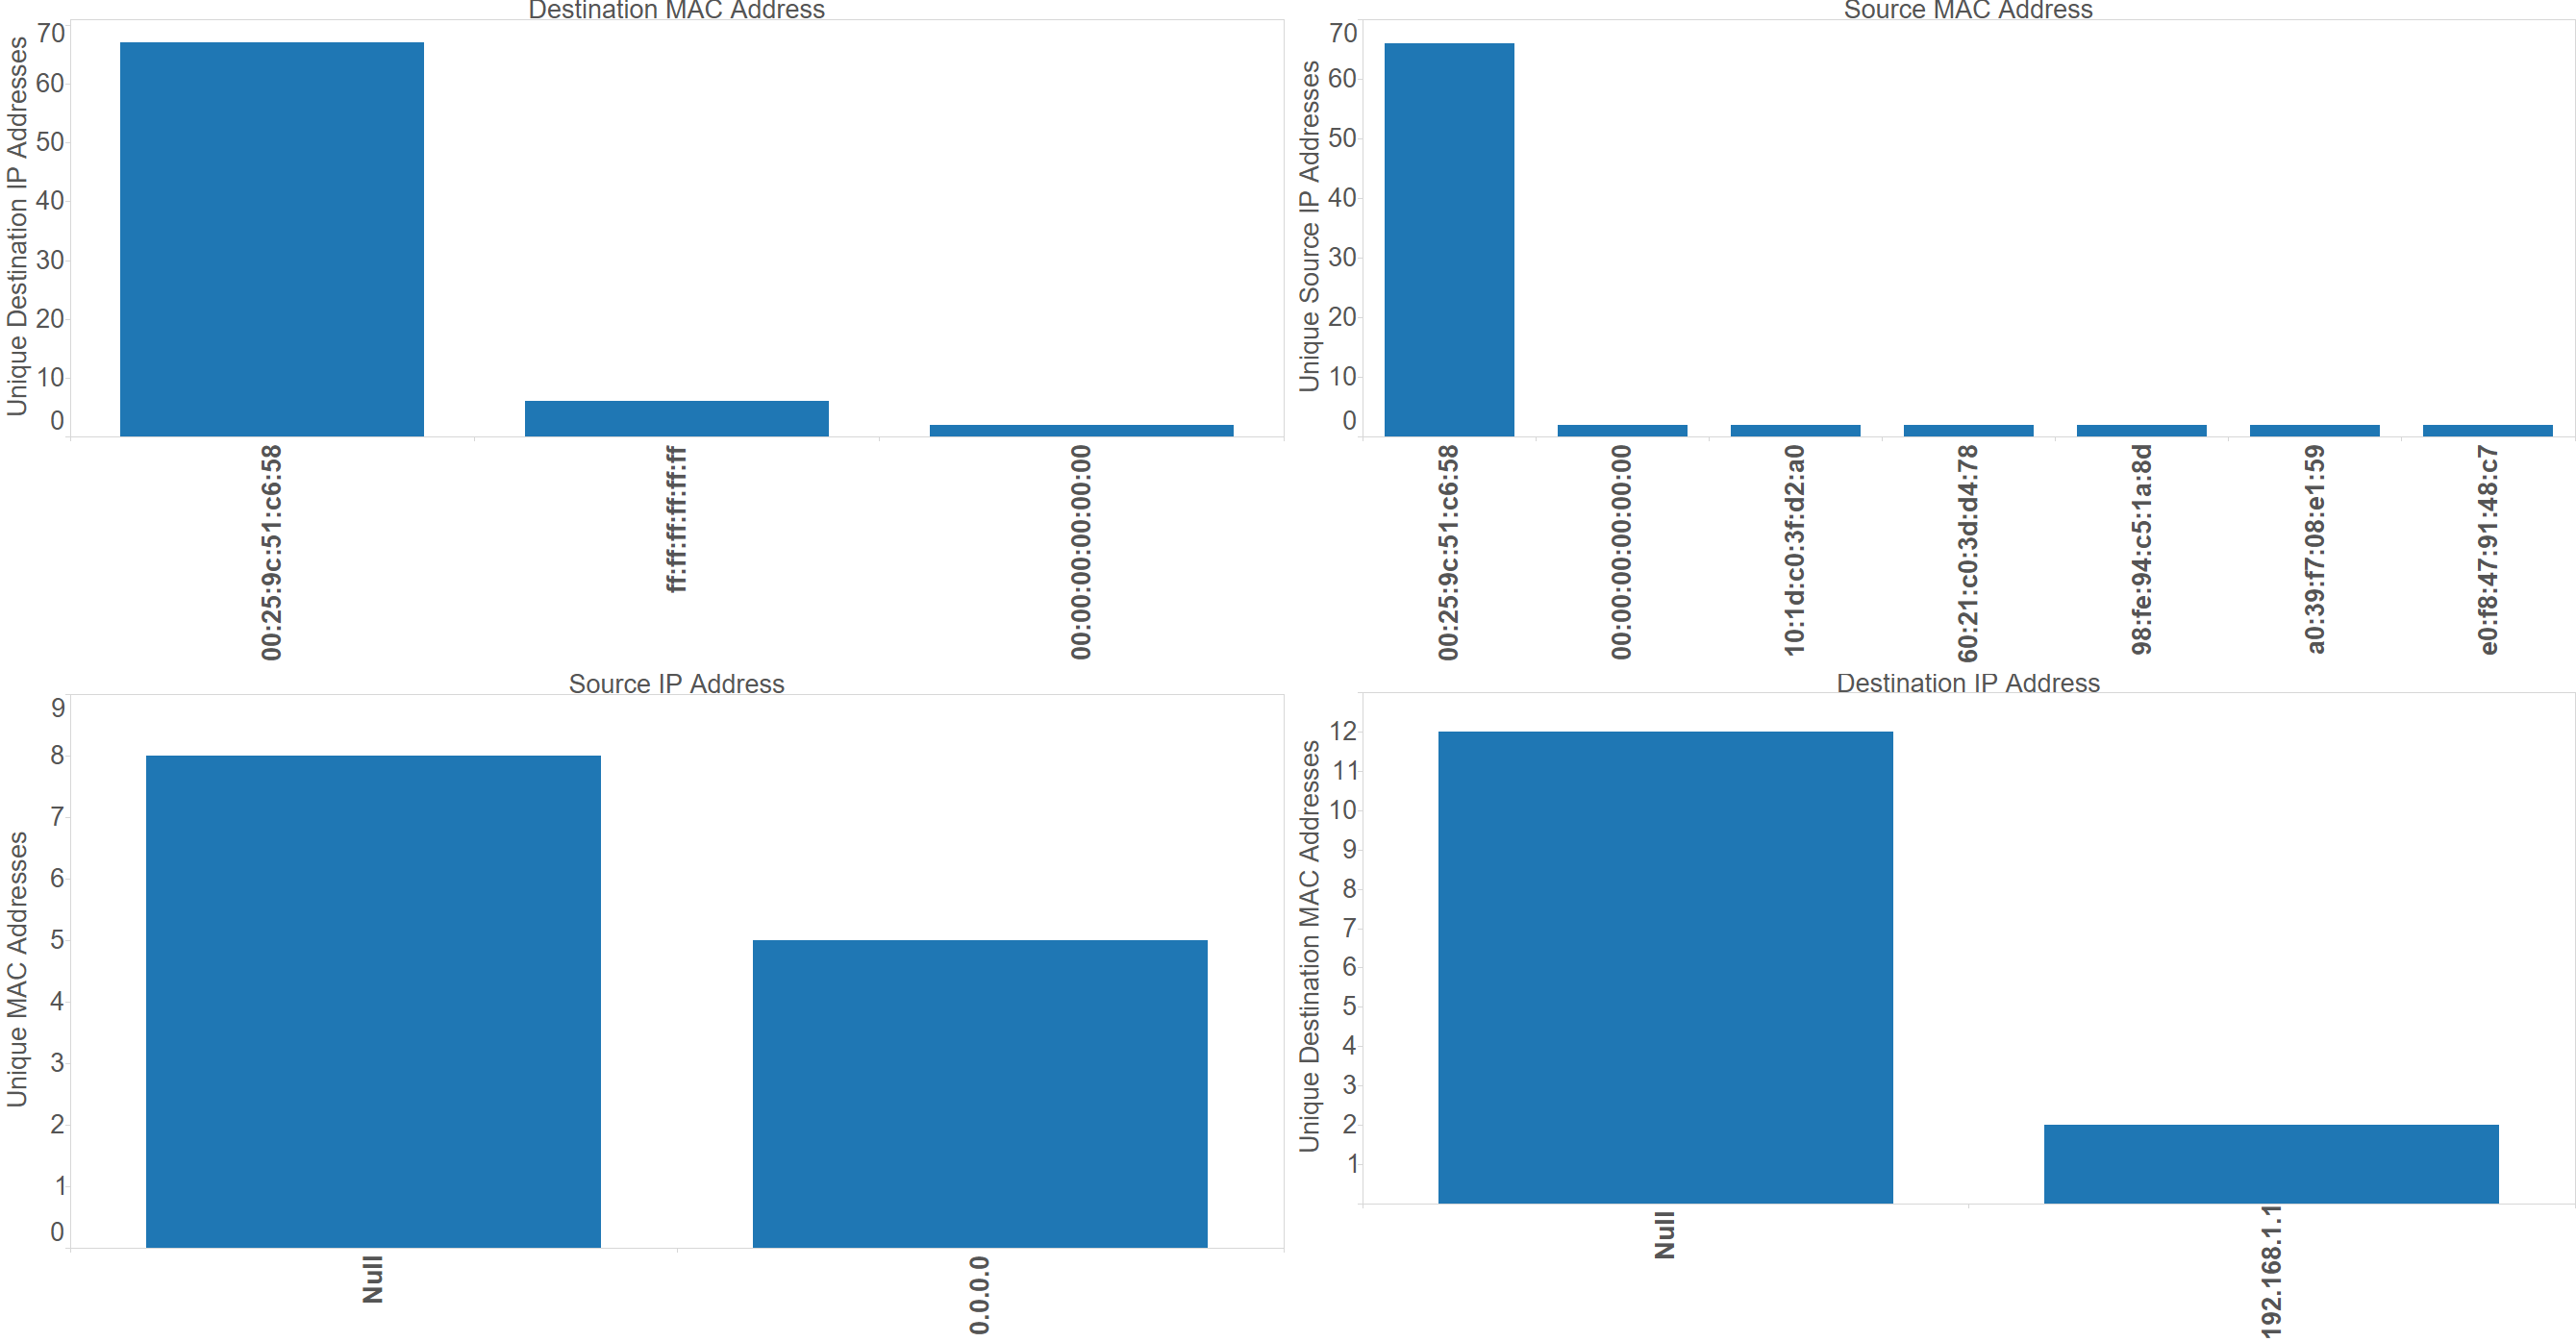
\includegraphics[width=1\textwidth]{../captures/CasaGerman/IP vs MAC Correspondence.png}
    \caption{Estos cuatro gráficos nos dan información sobre la relación entre las IP y Mac Addresses.}
    \label{fig:mesh1}
\end{figure}

El gráfico que se encuentra en la esquina superior izquierda nos muestra la cantidad de IP's distintas a las cuales fueron dirigidos paquetes provenientes de las Mac Addresses mostradas. El de la derecha por el contrario, nos muestra la cantidad de paquetes de distintas IP's que tienen por destino una misma Mac Address. La Mac Address que más recibe y más envía es 00:25:9c:51:c6:58 y casualmente corresponde al router (corroborado con el comando arp -n de Ubuntu). La dirección de broadcast (ff:ff:ff:ff:ff:ff) también se hace notar un poco en el primer gráfico. Esto último es razonable ya que es la que se encarga de enviar paquetes a todos los dispositivos de la red y por lo tanto va a tener tantas IP's distintas de destino como dispositivos conectados a la red con una IP asignada válida existan.
\par En cuanto a los gráficos de abajo, el de la izquierda nos dice, dada una IP, cuantas Mac Addresses distintas tuvieron dicha IP como fuente en los paquetes capturados. El gráfico de la derecha nos dice la cantidad de Mac Addresses distintas que aparecieron en paquetes enviados a una misma IP. Sin embargo, estos dos gráficos no nos dan mucha información debido a que por motivos que tienen que ver con la implementación de Scapy, sucede que para todos los paquetes cuyos protocolos son IPv6 o cualquier otro que no mencionamos en este informe, no es posible conseguir la dirección de IP. Las IP ``válidas'' que aparecen son solo dos, una es el router (192.168.1.1) y la otra es 0.0.0.0 que se utiliza cuando no se tiene asignado todavía una IP (por eso válidas entre comillas).

\section{Conclusiones}

Pudimos observar que, por lo general, las redes analizadas tienden a "distinguir" ciertos nodos como los que más tráfico generan (y reciben), estos suelen ser los Gateways que permiten conectarse a internet. No es una sorpresa esto, ya que en general, y en particular en los tipos redes wifi que analizamos (excluyendo el caso de Mercadolibre, que es más relativo), las redes wifi no suelen ser usadas tanto para conectar dispositivos dentro de la misma red, sino para proveer acceso a Internet.


El hecho de hacer un experimento sobre una red controlada, como punto de comparación con las otras 3 redes (una semi-controlada, la de mercadolibre, y las otras dos públicas y libres), nos permitió poder corroborar algunas de las hipótesis y forzar ciertas condiciones sobre la misma antes de comenzar la captura que no hubiera sido posible hacerlo con redes no controladas como las anteriores. En redes caseras como esta vemos que el router tiene una incidencia importante y el tráfico de paquetes suele ser reducido. En particular la cantidad de paquetes ARP fue muy reducida (incluso reseteando el router antes de comenzar las capturas) y los de IPv4 predominaron.

Esto puede ser debido a varias razones:
\begin{itemize}
 
\item Los distintos nodos conectados suelen guardar las direcciones MAC ya conocidas en una caché, en consecuencia no suele ser necesario recurrir a los protocolos ARP de manera frecuente.

\item Por otro lado, también ocurre que no suele haber mucho movimiento en los nodos en una red wifi controlada y no pública (refiriéndonos a movimiento como ingreso de nodos nuevos de manera seguida). Esto contrasta de manera clara con los experimentos de redes públicas, en los que podemos suponer que hay una clara relación entre el movimiento de la gente por el espacio que provee dicha red y los dispositivos que se conectan a la red provista.

\end{itemize}


    

\end{document}